% This work is licensed under the Creative Commons
% Attribution-NonCommercial-ShareAlike 4.0 International License. To view a copy
% of this license, visit http://creativecommons.org/licenses/by-nc-sa/4.0/ or
% send a letter to Creative Commons, PO Box 1866, Mountain View, CA 94042, USA.

\section{Verteilungskonvergenz im Raum stetiger Funktionen} %7
Sei $I:=[a,b]$ mit $a<b$ und
\begin{align*}
	C:=C(I):=\big\lbrace f:I\to\R\mid f\text{ stetig}\big\rbrace
\end{align*}
versehen mit der Supremumsmetrik
\begin{align*}
	d(f,g)&:=\sup\limits_{t\in I}\big|f(t)-g(t)\big|\qquad\forall f,g\in C.
\end{align*}
Gemäß Beispiel \ref{beisp2.6} ist $(C,d)$ separabel. 
Die durch $d$ induzierte Borel-$\sigma$-Algebra
%\begin{align*}
$\B(C):=\B_d\big(C(I)\big)$
%\end{align*}
gestattet einfache Beschreibung. 
Dazu:

\begin{definition}\ %7.1
	\begin{enumerate}[label=(\arabic*)]
		\item Sei $t\in I$. Die Abbildung 
		\begin{align*}
			\pi_t:C\to\R,\qquad\pi_t(f):=f(t)\qquad\forall f\in C
		\end{align*}
		heißt \textbf{Projektion in $t$}.
		\item Sei $T:=\big\lbrace t_1,\ldots,t_k\big\rbrace\subseteq I,k\in\N$. Die Abbildung
		\begin{align*}
			\pi_T:C\to\R^k,\qquad \pi_T(f):=\Big(f(t_1),\ldots,f(t_k)\Big)=:
			\Big(f(t)\Big)_{t\in T}\qquad\forall f\in C
		\end{align*}
		heißt \textbf{Projektion in $T$}.
	\end{enumerate}
\end{definition}

\begin{satz}\label{satz7.2}
	\begin{align*}
		\B(C)
		=\sigma\Big(\pi_t:t\in I\Big)=\sigma\Big(\pi_T:T\subseteq I,T\text{ endlich}\Big)
		%=\sigma\Big(\big\lbrace \pi_t^{-1}(B):t\in I,B\in\B(\R)\big\rbrace\Big)
	\end{align*}
	"kleinste $\sigma$-Algebra, sodass alle $\pi_t$ messbar sind"
\end{satz}

\begin{erinnerung}
	\begin{align*}
		\sigma\Big(\pi_t:t\in I\Big)
		\overset{\Def}&{=}
		=\sigma\Big(\big\lbrace \pi_t^{-1}(B):t\in I,B\in\B(\R)\big\rbrace\Big)\\
		\sigma\Big(\pi_T:T\subseteq I,T\text{ endlich}\Big)
		\overset{\Def}&{=}
		\sigma\Big(\big\lbrace \pi_T^{-1}(B):T\subseteq I\text{ endlich, }B\in\B(\R)\big\rbrace\Big)\\
		\sigma\colon\Potenzmenge{\Potenzmenge{\Omega}}\to\Potenzmenge{\Potenzmenge{\Omega}},\qquad 
		\sigma(\mathcal{M})&:=\bigcap\limits_{\begin{subarray}{c}
			\A\subseteq\Potenzmenge{\Omega}~\sigma\text{-Algebra}\\
			\mathcal{M}\subseteq\A
		\end{subarray}}
		\A
	\end{align*}
\end{erinnerung}

\begin{proof}
	Da $\pi_t=\pi_{\lbrace t\rbrace}$ und $T=\lbrace t\rbrace$, folgt
	\begin{align}\label{eqProof7.2(1)}\tag{1}
		\sigma\Big(\pi_t:t\in I\Big)
		\subseteq\sigma\Big(\pi_T:T\subseteq I\text{ endlich}\Big)
	\end{align}
	Weiterhin gilt:
	\begin{align*}
		&\big\Vert\pi_T(f)-\pi_T(g)\big\Vert_\infty
		=\max\limits_{1\leq i\leq k}\big|f(t_i)-g(t_i)\big|
		\leq d(f,g)\qquad\forall f,g\in C,\forall T=\lbrace t_1,\ldots,t_k\rbrace\subseteq I\\
		&\implies\pi_T:(C,d)\to\R^d\text{ ist stetig}
	\end{align*}
	Aus Satz \ref{Lemma3.2} (2) folgt, dass $B_T:\B(C)\to\B(\R^k)$ messbar ist für alle endlichen Teilmengen $T\subseteq I$. 
	Da $\sigma\big(\pi_T:T\subseteq I\text{ endlich}\big)$ die \ul{kleinste} $\sigma$-Algebra auf $C$ ist, bzgl. der \ul{alle} $\pi_T,T\subseteq I$ endlich, messbar sind, folgt
	\begin{align}\label{eqProof7.2(2)}\tag{2}
		\sigma\Big(\pi_T:T\subseteq I,T\text{ endlich }\Big)\subseteq\B(C)
	\end{align}
	Wegen \eqref{eqProof7.2(1)} und \eqref{eqProof7.2(2)} bleibt zu zeigen:
	\begin{align}\label{eqProof7.2(3)}\tag{3}
		\B(C)\subseteq\sigma\Big(\pi_t:t\in I\Big)
	\end{align}
	Dazu sei $G\in\G(C)$, d.h. $G\subseteq C$ offen. 
	Gemäß Satz \ref{satz2.9} existieren $f_i\in C$, $\varepsilon_i>0$, $i\in\N$ mit
	\begin{align}\label{eqProof7.2(4)}\tag{4}
		G=\bigcup\limits_{i\in\N}B\big(f_i,\varepsilon_i\big)\text{ (offene Kugel)}.
	\end{align}
	Für jede offene Kugel
	\begin{align}\label{eqProof7.2(5)}\tag{5}
		B(f,\varepsilon)
		&=\big\lbrace g\in C:d(g,f)<\varepsilon\big\rbrace
		=\bigcup\limits_{k\in\N}\underbrace{\left\lbrace g\in C:d(g,f)\leq\varepsilon-\frac{1}{k}\right\rbrace}_{=\text{ abgeschlossene Kugel}}
	\end{align}
	Betrachte daher eine beliebige \ul{abgeschlosssene} Kugel
	\begin{align*}
		\overline{B}(f,\delta)
		&=\Big\lbrace g\in C:\sup\limits_{t\in I}\big|g(t)-f(t)\big|\leq\delta\Big\rbrace\\
		&=\Big\lbrace g\in C:\sup\limits_{t\in I\cap\Q}\big|g(t)-f(t)\big|\leq\delta\Big\rbrace\\
		&=\bigcap\limits_{t\in I\cap\Q}\Big\lbrace g\in C:\big|g(t)-f(t)\big|\leq\delta\Big\rbrace\\
		&=\bigcap\limits_{t\in I\cap\Q}\underbrace{\Big\lbrace g\in C:f(t)-\delta\leq \overbrace{g(t)}^{=\pi_t(g)}\leq f(t)+\delta\Big\rbrace}_{\pi_t^{-1}\Big(\big[f(t)-\delta,f(t)+\delta\big]\Big)\in\tilde{\B}}\\
		&\implies
		\overline{B}(f,\delta)\in\tilde{\B}\qquad\forall f\in C,\forall\delta>0\\
		&\stackrel{\eqref{eqProof7.2(5)}}{\implies}
		B(f,\varepsilon)\in\tilde{\B}\qquad\forall f\in C,\forall\varepsilon>0\\
		&\stackrel{\eqref{eqProof7.2(4)}}{\implies}
		G\in\tilde{\B}\\
		&\implies
		\G(C)\subseteq\tilde{\B}\\
		&\implies\sigma\big(\G(C))=\B(C)\subseteq\tilde{\B}
	\end{align*}
\end{proof}
%Ferger hat Borel-Mengen am Anfang des Studiums gehasst, weil er sie nicht verstanden hat. Jetzt sieht er das anders.

\begin{defi}
	Ein stochastischer Prozess $\big\lbrace X(t):t\in I\big\rbrace$ heißt \textbf{indiziert nach $I$ (über $(\Omega,\A)$)}
		\begin{align*}
	:\Longleftrightarrow X(t):(\Omega,\A)\to(\R,\B(\R)),
		\qquad\omega\mapsto X(t)(\omega)\quad
		\text{ist messbar}\qquad\forall t\in I
	\end{align*}
	%Ferger: "Trage ich zu einer Verwirrung bei?"
	Schreibweise: $X(t,\omega):=X(t)(\omega)$\\
	Falls die \textbf{Pfade / Trajektorien}
	\begin{align*}
		X(\cdot,\omega):I\to\R,\qquad t\mapsto X(t,\omega)\qquad\forall \omega\in\Omega
	\end{align*}
	stetig sind (für alle $\omega\in\Omega$), so liefert die Zuordnung $\omega\mapsto X(\cdot,\omega)$ eine Abbildung $X:\Omega\to C(I)$. 
	Diese Abbildung $X$ heißt \textbf{Pfadabbildung} des stochastischen Prozesses und wird mit diesem identifiziert, genauer:\\
	Für einen stochastischen Prozess $X\colon I\times\Omega\to\R$ gilt:
	\begin{itemize}
		\item $X\colon I\to\R,\qquad t\mapsto X(t,\omega)$ heißt \define{Pfad} für jedes $\omega\in\Omega$
		\item $X\colon\Omega\to\R,\qquad\omega\mapsto X(t,\omega)$ ist eine einzelne ZV für jedes $t\in I$
		\item $X\colon\Omega\to (I\to\R),\qquad \omega\mapsto(t\mapsto X(t,\omega))$ heißt \define{Pfadabbildung}
		\item Falls alle Pfade stetig (also $X$ ein \define{stetiger stochastischer Prozess} ist) sind, gilt $I\to\R=C(I)$.
		\item Man kann einen (stetigen) stochastischen Prozess mit seiner Pfadabbildung identifizieren:
		\begin{align}\label{eqIdentifiereSP}
			\big\lbrace X(t)\mid t\in I, X(t)\colon\Omega\to\R\big\rbrace
			\cong X\colon\Omega\to C(I)
		\end{align}
	\end{itemize}
\end{defi}

Satz \ref{satz7.2} liefert ein sehr handliches Kriterium für die Messbarkeit von allgemeinen Abbildungen $X:\Omega\to C$.

\begin{satz}\label{satz7.3}
	Sei $(\Omega,\A)$ messbarer Raum und $C:=C(I)$ versehen mit der Borel-$\sigma$-Algebra $\B(C)$ sowie $X:\Omega\to C$. Dann gilt:
	\begin{align*}
		X\text{ ist }A\text{-}\B(C)\text{-messbar}\Longleftrightarrow\forall t\in I:\pi_t\circ X\text { ist }\A\text{-}\B(R)\text{-messbar}
	\end{align*}
\end{satz}

\begin{proof}
	Erinnere an das Messbarkeitslemma:\nl
	\textbf{Lemma. (Messbarkeitslemma)}\\
	Sei $(\Omega,\A)$ messbarer Raum, $\Omega\neq\emptyset$, $(f_t)_{t\in T}$ eine Familie von Abbildungen\\ $f_t:\Omega\to(\Omega_t,\A_t)$ wobei $(\Omega_t,\A_t)$ messbarer Raum für alle $t\in T$, $T\neq\emptyset$ beliebige Indexmenge. 
	Ferner sei
	\begin{align*}
		\A':=\sigma\big(f_t:t\in T\big)\stackeq{\text{Def}}\sigma\left(\bigcup\limits_{t\in T} f_t^{-1}(\A_t)\right)
	\end{align*}
	Dann gilt für eine Abbildung $Z:\Omega\to\Omega'$:
	\begin{align*}
		Z\text{ ist }\A\text{-}\A'\text{-messbar}\Longleftrightarrow\forall t\in T: f_t\circ Z\text{ ist }\A\text{-}\A_t\text{-messbar}
	\end{align*}
	Im Falle von Satz \ref{satz7.3}: $\Omega'=C, f_t=\pi_t, T=I,\A'=\sigma\big(\pi_t:T\in I\big)\stackeq{\ref{satz7.2}}\B(C),Z=X$
\end{proof}

Stochastische Prozesse mit stetigen Pfaden nennt man \textbf{stetige} stochastische Prozesse. 
Satz \ref{satz7.3} besagt nun: 
Die Pfadabbildung eines jeden stetigen stochastischen Prozesses ist $\A\text{-}\B(C)$-messbar. 
Insbesondere folgt:\\
Jeder stetige stochastische Prozess indiziert nach $I$ kann aufgefasst werden als Zufallsvariable im metrischen Raum $\big(C(I),d\big)$.

\begin{beispiel}\label{beispiel7.4}
	Sei $(\xi_i)_{i\in\N}$ eine Folge von reellen Zufallsvariablen über $(\Omega,\A)$ und für $n\in\N$ sei
	\begin{align*}
		S_k:=\sum\limits_{i=1}^k\xi_i\qquad\forall0\leq k\leq n\qquad S_0:=0
	\end{align*}
	Der Polygonzug $X_n$ durch die Punkte $\left(\frac{k}{n},\frac{1}{\sqrt{n}}\cdot S_k\right),0\leq k\leq n$ heißt \textbf{$n$-ter Partialsummenprozess}.
	\begin{figure}[H]
		\begin{center}
			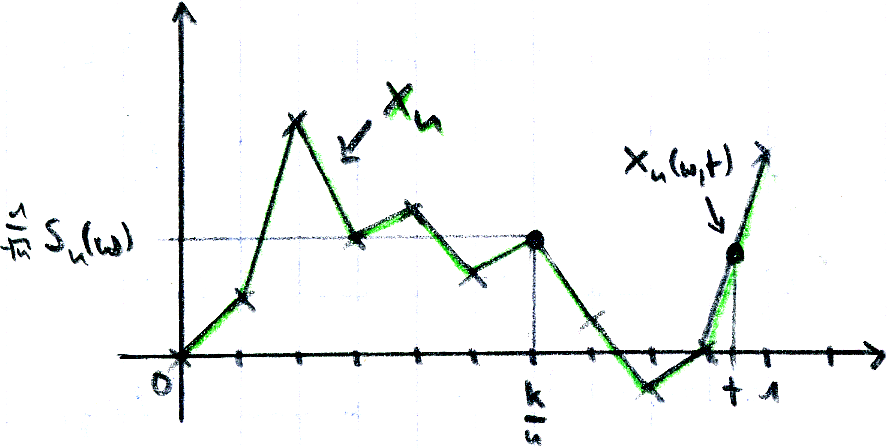
\includegraphics[width=1\textwidth]{./pics/MSTAT001.png}
			\caption{Partialsummenprozess mit $n=10$, $k=6$}
			\label{AbbPartialsummenprozess}
		\end{center}
	\end{figure}
	Mit der Zwei-Punkte-Formel der Geradengleichung folgt:
	\begin{align*}
		X_n(t)=\frac{1}{\sqrt{n}}\cdot\sum\limits_{i=1}^{\lfloor n\cdot t\rfloor}\xi_i+\frac{1}{\sqrt{n}}\cdot\big(n\cdot t-\lfloor n\cdot t\rfloor\big)\cdot\xi_{\lfloor n\cdot t\rfloor+1}\qquad\forall t\in[0,1]=I
	\end{align*}
	Hierbei ist die Gaußklammer (Abrundefunktion) wie folgt definiert:
	\begin{align*}
		\lfloor u\rfloor:=[u]:=\max\big\lbrace l\in\Z:l\leq n\big\rbrace
	\end{align*}
	$X_n(t)$ ist eine reelle Zufallsvariable für alle $t\in I$. 
	Gemäß Konstruktion (Polygonzug) ist jeder Pfad von $X_n$ stetig auf $[0,1]$. 
	Aus Satz \ref{satz7.3} folgt, dass $X_n~\A\text{-}\B(C)$-messbar ist, also Zufallsvariable in $\Big(C\big([0,1]\big),d\Big)$. 
	Weitere Anwendung von Satz \ref{satz7.2}:
\end{beispiel}

\begin{satz}\label{satz7.5}\
	\begin{enumerate}[label=(\arabic*)]
		\item $P,Q$ seien Wahrscheinlichkeitsmaße auf $\B(C)$. Dann gilt:
		\begin{align*}
			P=Q\Longleftrightarrow\forall T\subseteq I\text{ endlich }: P\circ\pi_T^{-1}=Q\circ\pi_T^{-1}
		\end{align*}
		\item $X,Y$ seien Zufallsvariablen in $\big(C(I),d\big)$. Dann gilt:
		\begin{align*}
			X\stackeq{\L}Y\Longleftrightarrow\forall T\subseteq I\text{ endlich }: \pi_T(X)\stackeq{\L}\pi_T(Y)
		\end{align*}
	\end{enumerate}
\end{satz}

\begin{proof}
	\underline{Zu (1), zeige ``$\implies$'':} Trivial.\nl
	\underline{Zu (1), zeige ``$\Longleftarrow$'':}\\
	Gemäß Satz \ref{satz7.2} ist
	\begin{align*}
		\mathcal{E}:=\left\lbrace\pi_T^{-1}(A):A\in\B(\R^{|T|},T\subseteq I\text{ endlich}\right\rbrace
	\end{align*}
	ein Erzeuger von $\B(C)$, d.h. $\B(C)=\sigma(\mathcal{E})$. Erinnerung:
	\begin{align*}
		g^{-1}(\mathcal{C})&:=\big\lbrace g^{-1}(C):C\in\mathcal{C}\big\rbrace\text{ für Mengenfamilie }\mathcal{C}\\
		\B(C)&\stackeq{\ref{satz7.2}}\sigma\big(\pi_T:T\subseteq I\text{ endlich}\big)
		=\sigma\Bigg(\underbrace{\bigcup\limits_{\begin{subarray}{c}T\subseteq I\\T\text{ endlich}\end{subarray}}\pi_T^{-1}\left(\B\left(\R^{|T|}\right)\right)}_{=\mathcal{E}}\Bigg)
	\end{align*}
	Nach Voraussetzung gilt:
	\begin{align*}
		\underbrace{P\circ\pi_T^{-1}(A)}_{\stackeq{\text{Def}}P\left(\pi_T^{-1}(A)\right)}&=\underbrace{Q\circ\pi_T^{-1}(A)}_{=Q\left(\pi_T^{-1}(A)\right)}\qquad\forall A\in\B\left(\R^{|T|}\right)\\
		\implies
		P|_\mathcal{E}&=Q|_\mathcal{E}
	\end{align*}
	$\mathcal{E}$ ist durchschnittsstabil (nachrechnen!). 
	Jetzt liefert der \textit{Maßeindeutigkeitssatz}, dass $P=Q$ auf $\sigma(\mathcal{E})=\B(C)$.
	(Der Maßeindeutigkeitssatz besagt ungefähr: 
	zwei Wahrscheinlichkeitsmaße, die auf einen Schnittstabilen Mengensystem überein stimmen, stimmen auch auf dessen Erzeugnis überein.)\nl
	\underline{Zeige (2):}
	\begin{align*}
		X\stackeq{\L} X
		\overset{\text{Def}}&{\Longleftrightarrow}
		\P\circ X^{-1}=\P\circ Y^{-1}\\
		\overset{(1)}&{\Longleftrightarrow}
		\underbrace{\left(\P\circ X^{-1}\right)\circ \pi_T^{-1}}_{=\P\circ\left(\pi_T\circ X\right)^{-1}}
		=\underbrace{\left(\P\circ Y^{-1}\right)\circ\pi_T^{-1}}_{=\P\circ\left(\pi_T\circ Y\right)^{-1}}
		&\forall T\subseteq T\text{ endlich}\\
		&\Longleftrightarrow
		\underbrace{\pi_T\circ X}_{=\pi_T(X)}\stackeq{\L}\underbrace{\pi_T\circ Y}_{=\pi_T(Y)}
		&\forall T\subseteq I\text{ endlich}
	\end{align*}
\end{proof}

\begin{bemerkungnr} %7.6
	Die Wahrscheinlichkeitsmaße $\P\circ\big(\pi_T\circ X)^{-1}$ bzw. die Verteilungen
	\begin{align*}
		\pi_T(X)&=\big(X(t_1),\ldots,X(t_k)\big)&\forall& T=\big\lbrace t_1,\ldots,t_k\rbrace\subseteq I\text{, genauer:}\\
		\pi_T\big(X(\omega)\big)&=\big(X(\omega)(t_1),\ldots,X(\omega)(t_k)\big)&\forall&\omega\in\Omega,\forall T=\big\lbrace t_1,\ldots,t_k\rbrace\subseteq I\\
		&\pi_T\circ X\colon\Omega\to C\to\R_k
	\end{align*}
	heißen \textbf{endlich dimensionale Randverteilungen von $\P$} bzw. von $X$.\\
	Insbesondere ist gemäß \ref{satz7.5} (2) die Verteilung eines stetigen stochastischen Prozesses $X$ aufgefasst als Zufallsvariable in $C$ eindeutig durch die Verteilungen der Vektoren
	\begin{align*}
		\big(X(t_1),\ldots,X(t_k)\big),\qquad t_1,\ldots,t_k\in I,k\in\N
	\end{align*}
	festgelegt.
\end{bemerkungnr}

Nächstes Ziel: Handhabbare Kriterien für den Nachweis der Verteilungskonvergenz in $C$. Dazu:

\begin{definition} %7.7
	Für eine Funktion $f\colon I\to\R$ und $\delta>0$ definiere den \textbf{Stetigkeitsmodul / Oszillationsmodul}
	\begin{align*}
		\omega(f,\delta):=\sup\limits\Big\lbrace \big|f(s)-f(t)\big|:s,t\in I\mit |s-t|\leq\delta\Big\rbrace
	\end{align*}
\end{definition}

Aus der Analysis ist bekannt:
\begin{align*}
	f\in C(I)\Longleftrightarrow\omega(f,\delta)\stackrel{\delta\to0}{\longrightarrow}0
\end{align*}

\begin{lemma}\label{lemma7.8}
	$\omega(\cdot,\delta)\colon (C,d)\to\R$ ist stetig für jedes $\delta>0$ und damit gemäß Lemma \ref{Lemma3.2} (2) auch $\B(C)$-$\B(\R)$-messbar.
\end{lemma}

\begin{proof}
	Sei $g\in C$ und $s,t\in I$ mit $|s-t|\leq\delta$. 
	Dann gilt:
	\begin{align*}
		\big| f(s)-f(t)\big|
		&=\big|f(s)-g(s)+g(s)-g(t)+g(t)-f(t)\big|\\
		\overset{\text{DU}}&{\leq}
		\underbrace{\big|f(s)-g(s)\big|}_{\leq d(f,g)}+\underbrace{\big| g(s)-g(t)\big|}_{\leq\omega(g,\delta)}+\underbrace{\big| g(t)-f(t)\big|}_{\leq d(f,g)}\\
		&\leq
		\omega(g,\delta)+2\cdot d(f,g)\\
		\overset{\sup}&{\implies}
		\omega(f,\delta)
		\leq\omega(g,\delta)+2\cdot d(f,g)\\
		&\implies \omega(f,\delta)-\omega(g,\delta)
		\leq 2\cdot d(f,g) &\forall f,g\\
		&\implies \omega(g,\delta)-\omega(f,\delta)
		\leq 2\cdot d(g,f)=2\cdot d(f,g)\\
		&\implies
		\big|\omega(f,\delta)-\omega(g,\delta)\big|\leq 2\cdot d(f,g)
	\end{align*}
	Das heißt, $\omega(\cdot,\delta)$ ist sogar Lipschitz-stetig.
\end{proof}

%Ferger: "Ich war übrigens gestern in der Stadt. Da bin ich eigentlich nie. Ich war in mindestens 7 oder Schuhgeschäften. Es war noch jemand dabei. Ich selber habe kein Schuhe gekauft. Und in jedem Geschäft war die Verweildauer sehr lang. Und jedes Schuhgeschäft wurde GESCANNT: Jeder Schuh wurde angefasst und begutachtet. [...] Weihnachten ist was Schönes!"

%Ferger: "Wenn man sich rote Schuhe kauft, muss dazu auch noch eine passende rote Tasche kaufen. Wussten Sie das?"

Erstes Kriterium in:

\begin{satz}\label{satz7.9}
	Seien $X,X_n,n\in\N$ Zufallsvariablen in $C$ über $(\Omega,\A,\P)$. Falls
	\begin{enumerate}[label=(\arabic*)]
		\item $\begin{aligned}
			\underbrace{\big(X_n(t_1),\ldots,X_n(t_k)\big)}_{=\pi_T\circ X_n}\stackrel{\L}{\longrightarrow}\underbrace{\big(X(t_1),\ldots,X(t_k)\big)}_{=\pi_T\circ X}
			\qquad\forall t_1,\ldots,t_k\in I,\forall k\in\N
		\end{aligned}$\\
		so genannte \textbf{Konvergenz der fidis} (finite dimensional distributions).\\
		Notation: $X_n\stackrelnew{\text{fd}}{}{\longrightarrow} X$
		\item $\begin{aligned}
			\lim\limits_{k\to\infty}\limsup\limits_{n\to\infty}\P\Big(\omega\big(X_n,\delta_k\big)>\varepsilon\Big)=0\qquad\forall\varepsilon>0
		\end{aligned}$\\
		für eine Folge $(\delta_k)_{k\in\N}\subseteq(0,\infty)\mit\delta_k\downarrow0$
	\end{enumerate}
	so folgt:
	\begin{align*}
		X_n\stackrel{\L}{\longrightarrow}X\text{ in }(C,d)
	\end{align*}
\end{satz}

\begin{proof}
	Siehe Gänssler und Stute (1977) \textit{Wahrscheinlichkeitstheorie}, Seite 348
\end{proof}

\begin{beispiel}\label{beispiel7.10} Sei 
	\begin{align*}
		X_n(t):=A_n+B_n\cdot t+C_n\cdot t^2\qquad\forall t\in I
		\qquad\mit \big(A_n,B_n,C_n)\stackrel{\L}{\longrightarrow}(A,B,C)\in\R^3
	\end{align*}
	Dann gilt:
	\begin{align*}
		X_n\stackrel{n\to\infty}{\longrightarrow} X\text{ in }(C,d)\qquad\mit\qquad X(t)=A+B\cdot t+C\cdot t^2
	\end{align*}
	
	\begin{proof}
		Seien $t_1,\ldots,t_k\in I$ beliebig. 
		Für Voraussetzung (1) in Satz \ref{satz7.9} reicht es gemäß Cramér-Wold-Device \ref{satz5.4CramerWoldDevice} zu zeigen:
		\begin{align*}
			\sum\limits_{j=1}^k\lambda_j\cdot X_n(t_j)\stackrel{\L}{\longrightarrow}\sum\limits_{j=1}^k\lambda_j\cdot X(t_j)\text{ in }\R\qquad\forall\lambda=\big(\lambda_1,\ldots,\lambda_k\big)\in\R^k
		\end{align*}
%Ich wurde von Prof Ferger bemitleidet, weil ich in Tex nicht alles umsetzen kann, was er an der Tafel durch Wisch-Technik erzeugt.
		Dazu: 
		\begin{align*}
			\sum\limits_{j=1}^k\lambda_j\cdot X_n(t_j)
			&=A_n\cdot\sum\limits_{j=1}^n\lambda_j+B_n\cdot\sum\limits_{j=1}^k\lambda_j\cdot t_j+C_n\cdot\sum\limits_{j=1}^k\lambda_j\cdot t_j^2\\
			\overset{\L,\ref{satz4.10ContinuousMappingTheorem}}&{\longrightarrow}
			A\cdot\sum\limits_{j=1}^k\lambda_j+B\cdot\sum\limits_{j=1}^k\lambda_j\cdot t_j+C\cdot\sum\limits_{j=1}^k\lambda_j\cdot t_j^2
			=\sum\limits_{j=1}^k\lambda_j\cdot X(t_j)
		\end{align*}
		Zu Voraussetzung (2) in Satz \ref{satz7.9}:
		\begin{align*}
			\big|X_n(s)-X_n(t)\big|
			&=\Big|B_n\cdot(s-t)+C_n\cdot\underbrace{\big(s^2-t^2\big)}_{(s-t)\cdot(s+t)}\Big|\\
			\overset{\text{DU}}&{\leq}
			|B_n|\cdot\underbrace{|s-t|}_{\leq\delta}+|C_n|\cdot\underbrace{|s-t|}_{\leq\delta}\cdot\underbrace{|s+t|}_{\leq|s|+|t|\leq:K}\\
			&\leq
			|B_n|\cdot\delta+K\cdot|C_n|\cdot\delta\qquad\forall s,t\in I\mit |s-t|\leq\delta\\
			\overset{\sup}{\implies}
			\omega(X_n,\delta)
			&\leq|B_n|\cdot\delta+K\cdot|C_n|\cdot\delta\\
			\implies
			\P\Big(\omega\big(X_n,\delta\big)>\varepsilon\Big)
			&\leq\P\Big(|B_n|\cdot\delta+K\cdot|C_n|\cdot\delta>\varepsilon\Big)\\
			\overset{\eqref{eqProofBeispiel7.10}}&{\leq}
			\P\Big(|B_n|\cdot\delta>\frac{\varepsilon}{2}\Big)+\P\Big(K\cdot|C_n|\cdot\delta>\frac{\varepsilon}{2}\Big)\\
			&=
			\P\Big(|B_n|>\frac{\varepsilon}{2\cdot\delta}\Big)+\P\Big(|C_n|>\frac{\varepsilon}{2\cdot K\cdot\delta}\Big)\\
			&=
			1-F_n\left(\frac{\varepsilon}{2\cdot\delta}\right)+1-G_n\left(\frac{\varepsilon}{2\cdot K\cdot\delta}\right)
		\end{align*}
%Ferger: "Warum habe ich das eigentlich so gemacht!?"
		Hierbei ist $F_n$ die Verteilungsfunktion von $|B_n|\stackrel{\L}{\longrightarrow}|B|$ und $G_n$ die Verteilungsfunktion von $|C_n|$.
		Erinnerung:
		\begin{align}\label{eqProofBeispiel7.10}
			\big\lbrace U+V>\varepsilon\big\rbrace\subseteq\left\lbrace U>\frac{\varepsilon}{2}\right\rbrace\cup\left\lbrace V>\frac{\varepsilon}{2}\right\rbrace
		\end{align}
		Mit Korollar \ref{korollar4.5} folgt, dass es eine Fologe $(\delta_k)_{k\in\N}$  mit $\delta_k\downarrow0$, 
		so dass $\frac{\varepsilon}{2\cdot\delta_k}$ und $\frac{\varepsilon}{2\cdot K\cdot\delta_k}$ Stetigkeitsstellen der jeweiligen Grenz-Verteilungfunktionen sind,
%Ferger: "Na gut, einen Nobelpreis für Literatur kriege ich jetzt nicht."
		\begin{align*}
			\limsup\limits_{n\to\infty}\P\Big(\omega\big(X_n,\delta_k\big)>\varepsilon\Big)\leq\P\Big(|B|>\underbrace{\frac{\varepsilon}{2\cdot\delta_k}}_{\stackrel{k\to\infty}{\longrightarrow}\infty}\Big)
			+\P\Big(|C|>\underbrace{\frac{\varepsilon}{2\cdot K\cdot\delta_k}}_{\stackrel{k\to\infty}{\longrightarrow}\infty}\Big)
			\qquad\forall k\in\N
		\end{align*}
%Ferger: "Hach ich bin so doof. Ich hätte mir das Leben leichter machen können."
		$k\to\infty$ liefert dann (2).\\
		\textbf{Aufgabe:} Zeige dieses Beispiel durch CMT \ref{satz4.10ContinuousMappingTheorem}.
	\end{proof}
\end{beispiel}
 
Zweite Möglichkeit für den Nachweis der Verteilungskonvergenz in $C$ liefert:

\begin{satz}[Momentenkriterium von Kolmogoroff]\label{satz7.11MomentenkriteriumVonKolmogoroff}\enter
	Seien $X,X_n,n\in\N$ Zufallsvariablen in $C$ mit
	\begin{align}\label{eqSatz7.11Vor1}\tag{1}
		X_n\stackrelnew{\text{fd}}{}{\longrightarrow} X\qquad\text{(vgl. (1) in Satz \ref{satz7.9})}
	\end{align}
	Falls es eine Konstante $\gamma>0$ und $\alpha>1$ sowie eine stetige und monoton wachsende Funktion $F:I\to\R$ gibt, derart, dass
	\begin{align}\label{eqSatz7.11VorM}\tag{M}
		\E\Big[|X_n(s)-X_n(t)|^\gamma\Big]\leq\big(F(s)-F(t)\big)^\alpha\qquad\forall s,t\in I\mit s>t
	\end{align}
	Dann gilt:
	\begin{align*}
		X_n\stackrel{\L}{\longrightarrow} X\text{ in }\big(C(I),d\big)
	\end{align*}
\end{satz}

\begin{proof}
	Siehe Billingsley (1968), \textit{Convergence of probability measures}, Seite 96.
%Ferger: "Das Buch hier war früher meine Fibel."
%Ferger: "Jim Morrison von den Doors. Das war mein Held. Neben Skorokott."
\end{proof}

\ul{Ziel:} Verteilungskonvergenz der Partialsummenprozesse $X_n$ aus dem Beispiel \ref{beispiel7.4}. 
Dazu:

\begin{definition}\label{def7.12} %7.12
	Sei $I=[0,b]\mit b>0$ und $B:=\big\lbrace B(t):=B(t,\omega)\in I\big\rbrace$ ein stetiger stochastischer Prozess über $(\Omega,\A,\P)$ mit 
	\begin{enumerate}[label=(\arabic*)]
		\item $\begin{aligned}
			B(0)=B(0,\omega)=0\qquad\forall\omega\in\Omega
		\end{aligned}$
		\item $\begin{aligned}
			\forall 0=:t_0\leq t_1<\ldots<t_r\leq b
		\end{aligned}$ sind die Zuwächse $B(t_i)-B(t_{i-1}),1\leq i\leq r$\\ \ul{unabhängig}
		\item $\begin{aligned}
			0\leq s<t\leq b\implies B(t)-B(s)\sim\mathcal{N}(0,t-s)
		\end{aligned}$
	\end{enumerate}
	Dann heißt $B$ \textbf{Brownsche Bewegung (BB)} auf $I$.\\
	Vollkommen analog definiert man eine BB auf $I=[0,\infty)$.
\end{definition}

%Ferger: "Das ist wie so ein Wunschzettel. Es gelte 1, 2 und 3. Passend zur Weihnachtszeit. Wenn's dumm läuft, kann es noch sein, dass mein Wunsch nicht erfüllt wird, weil er nicht erfüllt werden kann."
%Ferger: "In der Hoffnung das Sie nicht schonmal hier gesessen haben: Weil ich immer dieselben Geschichten erzähle. Ich bin jetzt in so einem Alter wo man alles mehrfach erzählt."
%Ferger: "Da hat mal jemand eine Doktorarbeit geschrieben über eine tolle Fukntionenklasse. Und dann kam jemand daher, dass die Funktionenklasse nur aus der Eins-Funktion besteht. Das war echt ein Griff ins Klo. Wäre noch heftiger gewesen, wenn die Funktionenklasse leer gewesen wäre. Aber: So sind wir ja auch alle gestrickt. So werden wir konditionert. Weil, wenn der Mathematiker irgendwas hört, fragt der Mathematiker ständig "Existiert das?""

\begin{satz}[Lévy]\label{satz7.13Levy}
	Eine BB existiert.
\end{satz}

\begin{proof}
	Siehe Vorlesung \textit{Stochastische Prozesse}.
%Ferger: "Es gibt einen konstruktiven Beweis, der ist auch lehrrreich, aber da haben wir jetzt keine Zeit für.
%Anmerkung des Autors: Geschichten erzhählen ist wohl wichtiger
\end{proof}

\begin{lemma}\label{lemma7.14}
	Sei $B$ eine BB auf $I$ und $t_1<\ldots<t_r$ aus $I$. Dann gilt:
	\begin{align*}
		\Big(B(t_1),\ldots, B(t_r)\Big)^T\sim\mathcal{N}_r(0,\Gamma)\text{ wobei }\\
		\Gamma:=\Big(\Cov\big(B(t_i),B(t_j)\big)\Big)_{1\leq i,j\leq r}=\big(t_i\wedge t_j\big)_{1\leq i,j,\leq r}
	\end{align*}
	% \wedge meint Minimum
\end{lemma}

\begin{proof}
	Sei $t_0:=0$. Dann gilt:
	\begin{align*}
		B(t_j)
		\overset{\text{\ref{def7.12}(1)}}=
		B(t_j)-\underbrace{B(t_0)}_{=0}
		\overset{\text{Teles}}{=}
		\sum\limits_{i=1}^j\big(B(t_i)-B(t_{i-1})\big)
		=\sum\limits_{i=1}^j\sqrt{t_i-t_{i-1}}\cdot\underbrace{\frac{B(t_i)-B(t_{i-1})}{\sqrt{t_i-t_{i-1}}}}_{=:Z_i}
	\end{align*}
	Da $B(t_i)-B(t_{i-1})\sim\mathcal{N}(0,t_i-t_{i-1})$ folgt, dass die $Z_i$ i.i.d. $\sim\mathcal{N}(0,1)$ sind.
	Also ist der Vektor
	\begin{align*}
		\begin{pmatrix}
			B(t_1)\\
			\vdots\\
			B(t_r)
		\end{pmatrix}&=\begin{pmatrix}
			\sqrt{t_1} & 0 & \hdots & \hdots & 0\\
			\sqrt{t_1} & \sqrt{t_2-t_1} & 0 & \hdots & 0\\
			\vdots & \vdots & \ddots & \ddots & \vdots\\
			\sqrt{t_1} & \sqrt{t_2-t_1} & \sqrt{t_3-t_2} & \hdots & 0\\
		\end{pmatrix}\cdot\begin{pmatrix}
			Z_1\\
			\vdots\\
			Z_r
		\end{pmatrix}\implies\begin{pmatrix}
			B(t_1)\\
			\vdots\\
			B(t_r)
		\end{pmatrix}\sim\mathcal{N}_r(\mu,\Gamma)\\
		\mu_i:&=\E\Big[B(T_i)\Big]=\E\Big[\underbrace{B(t_i)-B(t_0)}_{\sim\mathcal{N}(0,t_i-t_0)}\Big]\qquad\forall i\\
		\implies\mu_i :&=\big(\mu_1,\ldots,\mu_r\big)=0
	\end{align*}
	Ferner sei $i\leq j$. Dann gilt:
	\begin{align*}
		\Cov\big(B(t_i),B(t_j)\big)
		&=\E\Big[B(t_i)\cdot B(t_j)\Big]\\
		&=\E\Big[B(t_i)\cdot\big( B(t_j)-B(t_i)+B(t_i)\big)\Big]\\
		&=\E\Big[\underbrace{B(t_i)\cdot\big(B(t_j)-B(t_i)\big)}_{\text{beide Faktoren sind unabh.}}+\big(B(t_i)\big)^2\Big]\\
		&=\E\Big[B(t_i)\cdot\big(B(t_j)-B(t_i)\big)\Big]+\E\Big[\big(B(t_i)\big)^2\Big]\\
		\overset{\text{unab}}&=
		\underbrace{\E\big[B(t_i)\big]}_{=}\cdot\underbrace{\E\big[B(t_j)-B(t_i)\big]}_{=0}+\underbrace{\E\Big[\big(B(t_i)\big)^2\Big]}_{=\Var\big(B(t_i)\big)}\\
		\overset{\text{Vert}}&=
		\Var\big(\mathcal{N}(0,t_i)\big)\\
		&=t_i\\
		\overset{i\leq j}&{=}
		t_i\wedge t_j
	\end{align*}
	Analog behandle den Fall $i\geq j$.
\end{proof}

\begin{korollar}\label{korollar7.15Folgerung}
	Die Verteilung einer BB ist eindeutig bestimmt. 
\end{korollar}

\begin{proof}
	Seien $B$ und $\tilde{B}$ zwei BBs (i.d.R. über unterschiedlichen Wahrscheinlichkeitsräumen definiert). Dann gilt:
	\begin{align*}
		B\stackeq{\L}\tilde{B}
		\overset{\ref{satz7.5}}&{\Longleftrightarrow}
		\big(B(t_1),\ldots,B(t_r)\big)^T\stackeq{\L}\big(\tilde{B}(t_1),\ldots,\tilde{B}(t_r)\big)^T
		&\forall t_1<\ldots<t_r\in I,\forall r\in\N\\
		\overset{\ref{lemma7.14}}&\Longleftrightarrow
		\mathcal{N}_r(0,\Gamma)=\mathcal{N}_r(0,\Gamma)
		&\forall t_1<\ldots<t_r\in I,\forall r\in\N
	\end{align*}
	Die letzte Aussage gilt aber, weil jede mehrdimensionale Normalverteilung $\mathcal{N}_r(\mu,\Gamma)$ eindeutig durch $\mu$ und $\Gamma$ festgelegt ist:
	\begin{align*}
		\mathcal{N}(\mu,\sigma^2)=\mathcal{N}(m,s^2)\Longleftrightarrow m=\mu\text{ und }s^2=\sigma^2
	\end{align*}
\end{proof}

Die Verteilung $\P\circ B^{-1}=:W$ von  einer Brownschen Bewegung $B$ heißt \textbf{Wiener-Maß} (nach Norbert Wiener).
%Ferger: "Absoluter Schlaukopf. Ein Ammi. Ein US-Amerikaner. Der hat 21 promoviert. Da wo wir noch mit den Klötzchen spielen, hat der schon promoviert."
\begin{align*}
	B:(\Omega,\A,\P)\to\Big(C(I),\B_d\big(C(I)\big)\Big)
\end{align*}
%Ferger: "Die Brownsche Bewegung wird genannt Brownsche Bewegeung, weil folgendes passiert ist: es gab einen schottischen Bonatiker. Der hat also eine Flüssigkeit genommen, z. B. Wasser und dann ganz kleine Pollenkörner oder Staubkörnchen, also so was ganz klitzekleines oder eie kleine Minischuppe in sein Töpfchen getan, in seine Flüssigkeit und hat draufgeguckt und gesagt "Boah, da ist ja was los." [...] Ja ich erzähl das so wie bei der Sendung mit der Maus, weil man das so gut versteht. [...] Und er stellt fest, dass da viel los ist. Die Beobachtung hatten andere Leute wohl auch schon gemacht. Die ersten Leute, jeder von denen hat sich natürlich gefragt: Was steckt dahinter? Die ersten Leute haben als erklärungsversuch gegeben, dass es biologische Energie in sich hat. Der Robert Braun hat gesagt: Nein, das ist nicht so. Können Sie ja mal googeln. Entscheidend ist Folgendes: Das war ca. 182?. Dann kam Albert Einstein und hat gesagt: Nenene bzw. jajaja, was hier passiert ist Folgendes: So eine Flüssigkeit besteht ja aus ganz vielen Molekülen, die in Bewegung sind. Und die schießen wie wild hin und her. Die Moleküle sind aber klitzeklitzeklein. Das kleine Teilchen ist aber im mirkoskopischen Bereich, also im Vergleich zu den Molekülen ein Riesen-Oschi. Und die kleinen Teilchen hauen die ganze Zeit dagegen. Der Einstein ist hergegangen und hat das für Physiker-Verhältnisse sehr mathematisch beschrieben. Der Wiener hat das nochmal auf saubere, mathematische Füße gestellt (Funtionenraum, Verteilungen und solche Sachen...) Die haben das ein oder andere wohl handwaving gemacht und Norbert Wiener hat das dann mal mathematisch sauberr gemacht. Deshalb heißt die Verteilung einer Brownschen auch Wiener Maß.
%Ferger: Sind ja immernoch 7 Minuten. Mist. Na da kann ich ja noch eine Geschichte erzählen. 

\begin{satz}[Donsker]\label{satz7.16Donsker}%\enter
	Seien $(\xi)_{i\in\N}$ i.i.d. mit $\E[\xi_1]=0$ und $\Var(\xi_1)=1$.
	\begin{align*}
		S_k&:=\sum\limits_{i=1}^k\xi_i&\forall& k\in\N_0\\
		X_n(t)&:=\frac{1}{\sqrt{n}}\cdot S_{\lceil n\cdot t\rceil}+\frac{1}{\sqrt{n}}\cdot\big(n\cdot t-\lceil n\cdot t\rceil\big)\cdot\xi_{\lceil n\cdot t\rceil+1} &\forall& t\in I=[0,b]
	\end{align*}
	$b>0$ fest), d.h. $X_n$ ist der Polygonzug durch die Punkte $\left(\frac{k}{n},\frac{1}{\sqrt{n}}\cdot S_k\right)_{0\leq k\leq b\cdot n}$. Dann gilt:
	\begin{align*}
		X_n\stackrel{\L}{\longrightarrow} B\text{ in }\big(C(I),d\big)
	\end{align*}
	wobei $B$ eine BB auf $I=[0,b]$.
\end{satz}

\begin{proof}
	Anwendung von Satz \ref{satz7.11MomentenkriteriumVonKolmogoroff}. 
	Zeige also dessen Voraussetzungen:\nl
	\underline{\eqref{eqSatz7.11Vor1} Zeige Konvergenz der fidis:}\\
	Seien $0\leq t_1<\ldots<t_r\leq b$. 
	Dann gilt:
	\begin{align*}
		\left\Vert\big(X_n(t_i)\big)_{1\leq i\leq r}-\left(\frac{1}{\sqrt{n}}\cdot\sum\limits_{j=1}^{\lceil n\cdot t_i\rceil}\xi_j\right)_{1\leq i\leq r}\right\Vert
		&=\Bigg(\sum\limits_{i=1}^r\underbrace{\left|X_n(t_i)-\frac{1}{\sqrt{n}}\cdot\sum\limits_{j=1}^{\lceil n\cdot t_i\rceil}\xi_j\right|^2}_{\frac{1}{\sqrt{n}}\cdot\underbrace{\big|n\cdot t_i-\lceil n\cdot t_i\rceil\big|}_{\leq1}\cdot\xi_{\lceil n\cdot t_i\rceil}}\Bigg)^{\frac{1}{2}}\\
		&\leq
		\frac{1}{\sqrt{n}}\cdot\left(\sum\limits_{i=1}^r\xi_{\lceil n\cdot t_i\rceil+1}^2\right)^{\frac{1}{2}}
		\implies\\
		\P\left(\left\Vert\big(X_n(t_i)\big)_{1\leq i\leq r}-\left(\frac{1}{\sqrt{n}}\cdot\sum\limits_{j=1}^{\lceil n\cdot t_i\rceil}\xi_j\right)_{1\leq i\leq r}\right\Vert\right)
		&\leq\P\left(\sum\limits_{i=1}^r\xi^2_{\lceil n\cdot t_i\rceil+1}>n\cdot\varepsilon^2\right)\\
		\overset{\text{Markov}}&\leq
		\frac{1}{n}\cdot\varepsilon^{-2}\cdot\sum\limits_{i=1}^r\underbrace{\E\left[\xi^2_{\lceil n\cdot t_i\rceil+1}\right]}_{=1~\forall i}\\
		&=
		\frac{1}{n}\cdot\varepsilon^{-2}\cdot r\stackrel{n\to\infty}{\longrightarrow}0\qquad\forall\varepsilon>0
	\end{align*}
	Folglich sind die beiden Folgen
	\begin{align*}
		\big(X_n(t_i)\big)_{1\leq i\leq r}\qquad\text{und}\qquad\left(\frac{1}{\sqrt{n}}\cdot\sum\limits_{j=1}^{\lceil n\cdot t_i\rceil}\xi_j\right)_{1\leq i\leq r}
	\end{align*}
	stochastisch äquivalent. 
	Wegen Cramér (Satz \ref{satz4.14Cramer}) genügt es
	\begin{align}\label{eqProof7.16fd}\tag{fd}
		\left(\frac{1}{\sqrt{n}}\cdot S_{\lceil n\cdot t_i\rceil}\right)_{1\leq i\leq r}\stackrel{\L}{\longrightarrow}\big(B(t_1),\ldots,B(t_r)\big)
	\end{align}
	zu zeigen. 
	Aber \eqref{eqProof7.16fd} ist äquivalent zu 
	\begin{align}\label{eqProof7.16Stern}\tag{$\ast$}
		\frac{1}{\sqrt{n}}\cdot\left(S_{\lceil n\cdot t_i\rceil}-S_{\lceil n\cdot t_{i-1}\rceil}\right)_{1\leq i\leq r}\stackrel{\L}{\longrightarrow}\big(B(t_i)-B(t_{i-1})\big)_{1\leq i\leq r}
	\end{align}
	denn:
	\begin{align*}
		h:\R^r\to\R^r,\qquad h(x_1,\ldots,x_r):=\big(x_1,x_2-x_1,x_3-x_2,\ldots,x_r-x_{r-1}\big)
	\end{align*}
	ist stetig auf $\R^r$ und hat stetige Inverse $h^{-1}$ mit 
	\begin{align*}
		h^{-1}(y_1,\ldots,y_r)=\big(y_1,y_1+y_2,\ldots,y_1+\ldots+y_r\big)
	\end{align*}
	Also ist \eqref{eqProof7.16fd} äquivalent zu \eqref{eqProof7.16Stern} gemäß CMT \ref{satz4.10ContinuousMappingTheorem}.\\
	Beachte wegen \undefine{Blockungslemma} sind die Komponenten $\frac{1}{\sqrt{n}}\cdot\left(S_{\lceil n\cdot t_i\rceil}-S_{\lceil n\cdot t_{i-1}\rceil}\right)_{1\leq i\leq r}$ \underline{unabhängig} und gemäß \ref{def7.12} (2) sind auch $\big(B(t_i)-B(t_{i-1})\big)$, $a\leq i\leq r$ unabhängig. 
	Somit ist gemäß Satz \ref{satz4.21} \eqref{eqProof7.16Stern} äquivalent zu 
	\begin{align}\label{eqProof7.16SternStern}\tag{$\ast\ast$}
		\frac{1}{\sqrt{n}}\cdot\left(S_{\lceil n\cdot t_i\rceil}-S_{\lceil n\cdot t_{i-1}\rceil}\right)
		\stackrel{\L}{\longrightarrow}
		\big(B(t_i)-B(t_{i-1})\big)\text{ in }\R\qquad\forall 1\leq i\leq r
	\end{align}
	Dazu setze $k_n:=\lceil n\cdot t_i\rceil-\lceil n\cdot t_{i-1}\rceil$. Dann gilt:
	\begin{align*}
		&\frac{1}{\sqrt{n}}\cdot\left(S_{\lceil n\cdot t_i\rceil}-S_{\lceil n\cdot t_{i-1}\rceil}\right)\\
		&=\frac{1}{\sqrt{n}}\cdot\sum\limits_{j=\lceil n\cdot t_{i-1}\rceil+1}^{\lceil n\cdot t_i\rceil}\xi_j
		=\frac{1}{\sqrt{n}}\cdot\sum\limits_{j=1}^{k_n}\xi_{\lceil n\cdot t_{i-1}\rceil+j}
		\overset{\L}{=}
		\frac{1}{\sqrt{n}}\cdot\sum\limits_{j=1}^{k_n}\xi_j\\
		&=\underbrace{\sqrt{\frac{k_n}{n}}}_{=\sqrt{\frac{\lceil n\cdot t_i\rceil-\lceil n\cdot t_{i-1}\rceil}{n}}}\cdot\frac{1}{\sqrt{k_n}}\cdot\sum\limits_{j=1}^{k_n}\xi_j\\
		&=\underbrace{\sqrt{\frac{\lceil n\cdot t_i\rceil-\lceil n\cdot t_{i-1}\rceil}{n}}}_{\stackrel{n\to\infty}{\longrightarrow}\sqrt{t_i-t_{i-1}}}\cdot\underbrace{\frac{1}{\sqrt{k_n}}\cdot\sum\limits_{j=1}^{k_n}\xi_j}_{\stackrelnew{\text{ZGWS}}{n\to\infty}{\longrightarrow}\mathcal{N}(0,1)}\stackrelnew{\ref{beisp4.18}(3)}{\L}{\longrightarrow}\sqrt{t_i-t_{i-1}}\cdot\mathcal{N}(0,1)
		\overset{\L}{=}\underbrace{\mathcal{N}(0,t_i-t_{i-1})}_{
		\overset{\ref{def7.12}}{=}B(t_i)-B(t_{i-1})}
	\end{align*}
	Damit ist Voraussetzung \eqref{eqSatz7.11Vor1} aus \ref{lemma7.14} gezeigt.\nl
	Wir zeigen \eqref{eqSatz7.11VorM} für $\gamma=4$ und $\alpha=2$, falls $\mu_4:=\E\big[\xi_1^4\big]<\infty$ (das ist eine stärkere Voraussetzung)\\
	Seien $s>t$ aus $I=[0,b]$. 
	Dann gilt:
	\begin{align}\label{eqProof7.16Plus}\tag{+}
		&X_n(s)-X_n(t)\\
		&=\frac{1}{\sqrt{n}}\cdot\sum\limits_{j=\lceil n\cdot t\rceil+1}^{\lceil n\cdot s\rceil}\xi_j+\frac{1}{\sqrt{n}}\cdot\big(n\cdot s-\lceil n\cdot s\rceil\big)\cdot\xi_{\lceil n\cdot s\rceil+1}
		-\frac{1}{\sqrt{n}}\cdot\big(n\cdot t-\lceil n\cdot t\rceil\big)\cdot\xi_{\lceil n\cdot t\rceil+1}\nonumber
	\end{align}
	Da 
	\begin{align}\label{eqProof7.16PlusPlus}\tag{++}
		\lceil n\cdot t\rceil\leq n\cdot t\leq\lceil n\cdot t\rceil+1\qquad\forall t\geq0
	\end{align}
	folgt
	\begin{align*}
		\frac{k}{n}\leq t<\frac{k+1}{n},\qquad\frac{l}{n}\leq s<\frac{l+1}{n},\qquad k=\lceil n\cdot t\rceil,\qquad l=\lceil n\cdot s\rceil
	\end{align*}
	\underline{Fall 1: $s-t\leq\frac{1}{n}$}
	\begin{enumerate}[label=(\roman*)]
		\item $s$ und $t$ liegen im selben Intervall $\left[\frac{k}{n},\frac{k+1}{n}\right)$
		\item $s$ und $t$ liegen in zwei aufeinanderfolgenden Intervallen $t\in\left[\frac{k}{n},\frac{k\cdot n}{n}\right]$, $s\in\left[\frac{k+1}{n},\frac{k+2}{n}\right)$
	\end{enumerate}
%Ferger: Habe ich schon erwähnt, dass ich in Deutsch richtig schlecht war?
	\ul{Fall (i)}: $\lceil n\cdot s\rceil=\lceil n\cdot t\rceil$ und
	\begin{align*}
		X_n(s)-X_n(t)
		&=\frac{1}{\sqrt{n}}\cdot(n\cdot s-n\cdot t)\cdot\xi_{\lceil n\cdot t\rceil+1}
		=\sqrt{n}\cdot(s-t)\cdot\xi_{\lceil n\cdot t\rceil+1}\\
		\implies
		\E\Big[\big|X_n(s)-X_n(t)\big|^4\Big]
		&=n^2\cdot(s-t)^4\cdot\mu_4
		=\mu_4\cdot(s-t)^2\cdot\underbrace{(s-t)^2}_{<\frac{1}{n^2}}\cdot n^2\\
		&\leq\mu_4\cdot(s-t)^2
	\end{align*}
%Ferger: Sie haben vielleicht mitbekommen es wird momentan von der Digitalisierung geredet. Und der Bund will 5 mrd € zur Verfügung stellen. Aber die Lehrer sagen: "Wir müssen die Kinder in das Zeitalter der Digitalisierung bringen". Gestern, ich lag gerade so auf meiner Couch mit einem Glas Wein und ein Journalist sagte dann "Man darf nicht zurück in die Kreidezeit (Lehrer an der Tafel)" Ich bin so kurz zusammengezuckt und habe mir gedacht: "Ach du scheiße, was machst du denn in Dresden..." Also es gibt tatsächlich Leite, die sich auch damit beschäftigen und sagen das ist Mühsam mit der Tafel. Aber indem man schreibt, beschäftigt man sich schon intensiver mit Stoff. 
%Ferger: Manchmal ist weniger mehr.
	\ul{Fall (ii):} $k=\lceil n\cdot t\rceil$ und $l=k+1=\lceil n\cdot s\rceil$. Dann folgt aus \eqref{eqProof7.16Plus}:
	\begin{align*}
		X_n(s)-X_n(t)
		&=\frac{1}{\sqrt{n}}\cdot\xi_{k+1}+\frac{1}{\sqrt{n}}\cdot\big(n\cdot s-(k+1)\big)\cdot\xi_{k+2}-\frac{1}{\sqrt{n}}\cdot(n\cdot t-k)\cdot\xi_{k+1}\\
		&=\sqrt{n}\cdot\left(s-\frac{k+1}{n}\right)\cdot\xi_{k+2}+\sqrt{n}\cdot\xi_{k+1}\cdot\left(\frac{k+1}{n}-t\right)
	\end{align*}

	\begin{lem}[$c_r$-Ungleichung]\enter
		Seien $a_1,\ldots,a_m\in\R$ (paarweise verschieden) und $r\geq 1$. Dann gilt:
		\begin{align}\label{eqCrUngleichung}\tag{$C_r$}
			\left|\sum\limits_{i=1}^m a_i\right|^r\leq c_r\cdot\sum\limits_{i=1}^m|a_i|^r\mit c_r:= m^{r-1}
		\end{align}
	\end{lem}

	\begin{proof}
		Sei $Z$ diskrete Zufallsvariable mit $\P(Z=a_i)=\frac{1}{m}$ für $1\leq i\leq m$. Dann gilt:
		\begin{align*}
			\big|\underbrace{\E[Z]}_{=\frac{1}{n}\cdot\sum\limits_{i=1}^m a_i}\big|^r
			\overset{\text{Jensen}}&\leq
			\underbrace{\E\Big[|Z|^r\Big]}_{=\frac{1}{m}\cdot\sum\limits_{i=1}^m|a_i|^r}
			\implies
			m^{-r}\cdot\left|\sum\limits_{i=1}^m a_i\right|^r\leq\frac{1}{m}\cdot\sum\limits_{i=1}^m|a_i|^r
		\end{align*}
	\end{proof}

	Mit $m=2$ und $r=4$ folgt:
	\begin{align*}
		\big|X_n(s)-X_n(t)\big|^4
		&\leq 8\cdot\bigg(n^2\cdot\xi^4_{k+2}\cdot\Big(\underbrace{s-\frac{k+1}{n}}_{\leq s-t}\Big)^4+n^2\cdot\xi^4_{k+1}\cdot\Big(\underbrace{\frac{k+1}{n}-t}_{\leq s-t}\Big)^4\bigg)\\
		\implies
		\E\left[\big|X_n(s)-X_n(t)\big|^4\right]
		&\leq 16\cdot\mu_4\cdot \underbrace{n^2\cdot(s-t)^2}_{\overset{\text{Fall 1}}{\leq} 1}\cdot(s-t)^2
		\leq
		16\cdot\mu_4\cdot(s-t)^2
	\end{align*}

	\underline{Fall 2: $s-t\geq\frac{1}{n}$}\\
	Aus \eqref{eqProof7.16Plus} und \eqref{eqCrUngleichung} mit $r=4$ und $m=3$ folgt wegen $\big|\lceil n\cdot s-\lceil n\cdot s\rceil\big|\leq1$:
	\begin{align*}
		\E\Big[\big|X_n(s)-X_n(t)\big|^4\Big]
		\overset{}&{\leq}
		27\cdot\left(\frac{1}{n^2}\cdot\E\left[\left|\sum\limits_{i=\lceil n\cdot t\rceil+1}^{\lceil n\cdot s\rceil}\xi_i\right|^4\right]+\underbrace{\frac{1}{n^2}}_{\leq(s-t)^2}\cdot\mu_4+\underbrace{\frac{1}{n^2}}_{\leq(s-t)^2}\cdot\mu_4\right)
	\end{align*}

	\begin{lem}[Momenten-Ungleichung]\enter
	Seien $\xi_1,\ldots,\xi_n$ i.i.d., zentriert mit $\mu_4:=\E[\xi_1^4]<\infty$ und $\mu_2:=\E[\xi_1^1]$. Dann gilt:
		\begin{align*}
			\E\left[\left|\sum\limits_{i=1}^n\xi_i\right|^4\right]=n\cdot\mu_4+3\cdot n\cdot(n-1)\cdot\mu_2^2
			\leq 4\cdot\mu_4\cdot n^2
		\end{align*}
	\end{lem}

	\begin{proof}
		Zeige zuerst das Gleichheitszeichen:
		\begin{align*}
			\E\left[\left|\sum\limits_{i=1}^n\xi_i\right|^4\right]
			&=\E\left[\left(\sum\limits_{i=1}^n\xi_i\right)^4\right]\\
			&=\E\left[\sum\limits_{1\leq i,j,k,l\leq n}\xi_i\cdot\xi_j\cdot\xi_k\cdot\xi_l\right]\\
			&=\sum\limits_{1\leq i,j,k,l\leq n}\underbrace{\E\Big[\xi_i\cdot\xi_j\cdot\xi_k\cdot\xi_l\Big]}_{=:\mu_{i,j,k,l}}
		\end{align*}
		Die Tupel $(i,j,k,l)\in\lbrace1,\ldots,n\rbrace^4$ mit mindestens drei verschiedenen Komponenten liefern $\mu_{i,j,k,l}=0$, 
		denn z. B. (verschiedene Buchstaben repräsentieren verschiedene Zahlen):
		\begin{align*}
			\mu_{i,j,k,j}
			&=\E\Big[\xi_i\cdot\xi_j\cdot\xi_k\cdot\xi_j\Big]
			=\E\Big[\xi_i\cdot\xi_j^2\cdot\xi_k\Big]=\underbrace{\E\big[\xi_i\big]}_{=0}\cdot\E\big[\xi_i^2\big]\cdot\E\big[\xi_k\big]
		\end{align*}
		Folglich reduziert sich die obige auf (!)
		\begin{align*}
			&\sum\limits_{i=1}^4\underbrace{\E\Big[\xi_i^4\Big]}_{=\mu_4}
			+6\cdot\sum\limits_{1\leq i\leq j\leq n}
			\underbrace{\E\Big[\xi_i^2\cdot\xi_j^2\Big]}_{=\mu_2^2}
			+\underbrace{\cdot\sum\limits_{1\leq i\leq j\leq n}\underbrace{\E\Big[\xi_i\Big]}_{=0}\cdot\E\Big[\xi_j^3\Big]+4\cdot\sum\limits_{1\leq i\leq j\leq n}\E\Big[\xi_i^3\Big]\cdot\underbrace{\E\Big[\xi_j\Big]}_{=0}}_{=0}\\
			&=n\cdot\mu_4+6\cdot\mu_2^2\cdot\underbrace{\begin{pmatrix}
			n\\ 2
			\end{pmatrix}}_{=\frac{n\cdot(n-1)}{2}}\\
			&=\underbrace{n}_{\leq n^2}\cdot\mu_4+3\dot n\cdot\underbrace{(n-1)}_{\leq n}\cdot\underbrace{\mu_2^2}_{=\big(\E[\xi_1^2]\big)^2\stackrel{\text{Jensen}}{\leq}\mu_4}\\
			&\leq 4\cdot n^2\cdot\mu_4
		\end{align*}
		Siehe auch \textit{Turkish Journal of Mathematics, Moment equalities via integer partitions} (2014) von Dietmar Ferger für mehr Hintergründe.
	\end{proof}

	Mit diesem Lemma folgt:
	\begin{align*}
		\frac{1}{n^2}\cdot\E\left[\left|\sum\limits_{i=\lceil n\cdot t\rceil+1}^{\lceil n\cdot s\rceil}\xi_i\right|^4\right]
		&=
		\frac{1}{n^2}\cdot\E\left[\left|\sum\limits_{i=1}^{\lceil n\cdot s\rceil-\lceil n\cdot t\rceil}\xi_{i+\lceil n\cdot t\rceil}\right|^4\right]\\
		&\leq
		\frac{1}{n^2}\cdot 4\cdot\mu_4\cdot\Big(\underbrace{\lceil n\cdot s\rceil-\overbrace{\lceil n\cdot t\rceil}^{>n\cdot t-1}}_{\leq\underbrace{ n\cdot s-n\cdot t}_{=n\cdot(s-t)}+\underbrace{1}_{\stackrel{\text{2. Fall}}{\leq}n\cdot(s-t)}\leq2\cdot n\cdot(s-t)}\Big)^2\\
		&\leq
		\frac{1}{n^2}\cdot 4\cdot\mu_4\cdot 4\cdot n^2\cdot(s-t)^2\\
		&=16\cdot\mu_4\cdot(s-t)^2\\
		\implies
		\E\Big[\big|X_n(s)-X_n(t)\big|^4\Big]
		&\leq 27\cdot18\cdot\mu_4\cdot(s-t)^2\qquad\forall s>t\in I\\
		&=\Big(F(s)-F(t)\Big)^2
	\end{align*}

	wobei $F(s):=\sqrt{27\cdot18\cdot\mu_4}\cdot s$. 
	Offenbar ist $F$ stetig und streng monoton wachsend auf $I=[0,b]$.
	Folglich ist \eqref{eqSatz7.11VorM} aus Satz \ref{satz7.11MomentenkriteriumVonKolmogoroff} erfüllt mit $\mu=4$ und $\alpha=2>1$.\nl
	Wir haben Donsker \ref{satz7.16Donsker} gezeigt, allerdings unter der \ul{stärkeren} Voraussetzung $\E\big[\xi_1^4]<\infty$. 
	Den allgemeinen Fall $\E[\xi_1^2]<\infty$ zeigt man mit der sogenannten \textit{Methode des Stutzens (truncation)}, 
	vergleiche Achim Klenke (2008) \textit{Wahrscheinlichkeitstheorie}
\end{proof}

%Ferger: Ich bin mit meinem Leben ja sehr zufrieden. [...] Das anstregendste als Professor ist das Tafelwischen. Ansonsten ist der Job leicht verdientes Geld. 

\setcounter{satz}{15}
\begin{bemerkungnr}\label{bemerkung7.16Einhalb} %7.16. Einhalb
%\begin{bemerkung}
	Unser Beweis lässt sich sofort übertragen auf Dreiecksschemata\\ 
	$\big\lbrace\xi_{i,n}:1\leq i\leq n,n\in\N\big\rbrace$ mit $\xi_{1,n},\ldots,\xi_{n,n}$ i.i.d. $\sim H$ (verteilt nach Verteilungsfunktion $H$), 
	wobei die Verteilungsfunktion $H$ nicht von $n$ abhängt und $\E\big[\xi_{i,n}\big]=0$ und $\E\big[\xi_{i,n}^4\big]<\infty$ und $\Var(\xi_{i,n})=1$. \nl
	Prokhorov (1956), \textit{Convergence of random processes and limit theorems in probability theory, Theory of Probability and its applications 1},
	Seite 157-214, zeigt, dass auch hier die Existenz zweiter Momente $\E\big[\xi_{i,n}^2\big]<\infty$ ausreicht.
%\end{bemerkung}
\end{bemerkungnr}

Seien $(\xi_i)_{i\geq1}$ i.i.d. $\sim F$ mit $\E\big[\xi_1\big]=\mu\in\R$ und $\sigma^2:=\Var(\xi_1)\in(0,\infty)$. 
Dann ist Donsker \ref{satz7.16Donsker} anwendbar auf die \textbf{standardisierten Zufallsvariablen}
\begin{align*}
	\tilde{\xi}_i:=\frac{\xi_i-\mu}{\sigma},\qquad\forall i\geq1
\end{align*}
Beachte: Die Grenzverteilung $W$ in Satz \ref{satz7.16Donsker} (also das Wiener-Maß) hängt \ul{nicht} von $F$ ab. 
Die Grenzverteilung ist also invariant unter $F$. Deshalb heißt Satz \ref{satz7.16Donsker} auch \textbf{Invarianzprinzip}. 
(Andere Formulierung: \textbf{Funktionaler Grenzwertsatz})\nl
Sei $h\colon C\big([0,b]\big)\to\R$ messbar und $W$-fast überall stetig. 
Dann gilt wegen Satz \ref{satz7.16Donsker} und \ref{satz4.10ContinuousMappingTheorem}:
\begin{align}\label{eqUnder7.16Eins}\tag{1}
	h(X_n)\stackrel{\L}{\longrightarrow} h(B)
\end{align}
Kennt man die Verteilung von $h(B)$ (=Funktional der Brownschen Bewegung, dazu existiert umfangreiche Literatur, z.B. Borodin und Salminen (2002),
\textit{Handbook of Brownian motion}), so auch die Grenzverteilung von $h(X_n)$. Dies macht man sich in der asymptotischen Statistik zunutze
(siehe Beispiel später).
Umgekehrt lässt sich oft die Grenzverteilung $h(W)$ für besonders einfache Verteilungfunktionen $F$ bestimmen.
\begin{align*}
	h\big(X_n\big)\stackrel{\L}{\longrightarrow}Z
	\overset{\eqref{eqUnder7.16Eins}~\&~\ref{lemma4.6Einhalb}}{\implies}
	h(B)=Z
\end{align*}
Damit ist der Satz \ref{satz7.16Donsker} von Donsker auch nützlich in der Wahrscheinlichkeitstheorie.

\subsection{Anwendung von Donsker in der Statistik}
\begin{notation}
	Sei $X$ eine reelle Zufallsvariable. Dann schreibe
	\begin{align*}
		X\sim(\mu,\sigma^2):\Longleftrightarrow\E[X]=\mu\qquad\text{und}\qquad\Var(X)=\sigma^2
	\end{align*}
\end{notation}

Wir betrachten das \define{Change-Point-Problem:}
% mit diesem Problem hat Ferger seine Uni-Karriere gestartet
$X_{1,n},\ldots,X_{n,n},n\in\N$ unabhängig mit 
\begin{align*}
	\left\lbrace\begin{array}{cl}
		X_{i,n}\text{ i.i.d.}\sim(\mu,\sigma^2), &\falls 1\leq i\leq\tau_n\\
		X_{i,n}\text{ i.i.d.}\sim(\nu,\tau^2), &\falls \tau_n< i\leq n
	\end{array}\right.
\end{align*}
wobei $\tau_n\in\lbrace1,\ldots,n\rbrace$ \ul{unbekannt} (der sogenannte \textbf{Change-point\\ (moment of change)}) 

\begin{align*}
	\underbrace{X_{1,n},\ldots,X_{\tau_n,n}}_{\text{i.i.d.}\sim(\mu,\sigma^2)}\qquad\underbrace{X_{\tau_n+1,n},\ldots,X_{n,n}}_{\text{i.i.d.}\sim(\nu,\tau^2)}
\end{align*}
\underline{Annahmen:} $\mu,\sigma^2$ bekannt, $\nu,\tau^2$ unbekannt, $\nu>\mu$\nl
\underline{Ziel:} Finde Test für 
$H_0:\tau_n=n$, d.h. es hat kein Wechsel stattgefunden vs. $H_1:1\leq\tau_n<n$. Dazu betrachte
\begin{align*}
	S_k:=S_{k,n}&:=\frac{1}{\sqrt{n}}\cdot\sum\limits_{i=1}^k\underbrace{\frac{X_{i,n}-\mu}{\sigma}}_{=:\xi_{i,n}}&\forall& 0\leq k\leq n\\
	\E[S_k]&=0\qquad	&\forall& 0\leq k\leq\tau_n
\end{align*}
da
\begin{align*}
	S_k&=S_{\tau_n}+\frac{1}{\sqrt{n}}\cdot\sum\limits_{i=\tau_n+1}^k\frac{X_{i,n}-\mu}{\sigma}
\end{align*}
folgt
\begin{align*}
	\E[S_k]
	&=0+\frac{1}{\sqrt{n}}\cdot\sum\limits_{i=\tau_n+1}^k\frac{\overbrace{\E[X_{i,n}]}^{=\nu}-\mu}{\sigma}
	=\frac{1}{\sqrt{n}}\cdot\big(k-\tau_n\big)\cdot\frac{\nu-\mu}{\sigma}\qquad\forall\tau_n<k\leq n
\end{align*}
%TODO 3x Plots einfügen
% 1. Plot von $(k,\E[S_k)]$ einfügen: für k\leq\tau_n ist es immer 0, für k>\tau_n wächst es monoton
% 2.Plot von $(k,S_k)$ einfügen: unter H_1: für k\leq\tau_n ist es ein "rumzappeln" um die X-Achse; für k>\tau_n gibt es dann einen "Drift" nach oben
% 3. Plot von $(k,S_k)$ einfügen, unter H_0: hier kein Drift nach oben, nur herumzappeln um die x_Achse

Planversibler Test:
$H_0$ verwerfen $:\Longleftrightarrow T_n:=\max\limits_{0\leq k\leq n} S_k>k_\alpha$\nl
\underline{Ziel:} Bestimme kritischen Wert $k_\alpha$

\begin{lemma}\label{lemma7.17}
	Sei $\underline{y}=\big(y_0,y_1,\ldots,y_n\big)\in\R^{n+1}$ und $h(\ul{y})$ der Polygonzug durch die Punkte $\left(\frac{k}{n},y_k\right)_{0\leq k\leq n}$. 
	Dann gilt:
	\begin{enumerate}[label=(\arabic*)]
		\item $\begin{aligned}
			\max\limits_{0\leq k\leq n}y_k=\max\limits_{0\leq t\leq 1} h(\ul{y})(t)
		\end{aligned}$
		\item $\begin{aligned}
			\max\limits_{0\leq k\leq n}\big|y_k\big|=\max\limits_{0\leq t\leq 1} \big|h(\ul{y})(t)\big|
		\end{aligned}$
		\item $\begin{aligned}
			\ul{y},\ul{z}\in\R^{n+1}\implies h\big(\ul{y}+\ul{z}\big)=h\big(\ul{y}\big)+h\big(\ul{z}\big)
		\end{aligned}$
	\end{enumerate}
\end{lemma}

\begin{proof}
	\underline{Zeige (1):}
	Gemäß der Zwei-Punkte-Formel gilt:
	\begin{align}\label{eqProof7.17Stern}\tag{$\ast$}
		h\big(\ul{y}\big)(t)
		&=y_{k-1}+\big(n\cdot t-(k-1)\big)\cdot\big(y_k-y_{k-1}\big)
		\qquad\forall t\in\left[\frac{k-1}{n},\frac{k}{n}\right],\forall 1\leq k\leq n
	\end{align}
	Da
	\begin{align*}
		h\big(\ul{y}\big)\left(\frac{k}{n}\right)\overset{\text{Def}}{=}y_k\qquad\forall 0\leq k\leq n
	\end{align*}
	gilt in (1) und (2) in jedem Fall "$\leq$". Umgekehrt sei $t\in[0,1]$ beliebig. Dann:
	\begin{align*}
		\exists 1\leq k\leq n:t\in\left[\frac{k-1}{n},\frac{k}{n}\right]
	\end{align*}
	\underline{Fall 1:} $y_k\geq y_{k-1}$\\
	Dann ist $h\big(\ul{y}\big)$ monoton wachsend auf $\left[\frac{k-1}{n},\frac{k}{n}\right]$ und es gilt
	\begin{align*}
		h\big(\ul{y}\big)(t)\leq h\big(\ul{y}\big)\left(\frac{k}{n}\right)=y_k\leq\max\limits_{0\leq k\leq n} y_k
	\end{align*}
	\underline{Fall 2:} $y_k<y_{k-1}$\\
	Dann ist $h\big(\ul{y}\big)$ monoton fallend und es gilt
	\begin{align*}
		h\big(\ul{y}\big)(t)\leq h\big(\ul{y}\big)\left(\frac{k-1}{n}\right)=y_{k-1}\leq\max\limits_{0\leq k\leq n}y_k
	\end{align*}

	\underline{Zeige (2):} In Fall 1 gilt:
	\begin{align*}
		h\big(\ul{y}\big)(t)&\leq y_k\leq\big|y_k\big|\leq\max\limits_{0\leq k\leq n}\big|y_k\big|\\
		h\big(\ul{y}\big)(t)&\geq y_{k-1}\geq-\big|y_{k-1}\big|\geq-\max\limits_{0\leq k\leq n}\big|y_k\big|\\
		\implies
		\Big|h\big(\ul{y}\big)(t)\Big|&\leq\max\limits_{0\leq k\leq n}\big| y_k\big|
	\end{align*}
	Fall 2 analog. Somit folgt (2).\nl
	\underline{Zeige (3):}\\
	Folgt aus \eqref{eqProof7.17Stern}.
\end{proof}

Es folgt aus dem Lemma \ref{lemma7.17} (1) (mit $y_k=S_k$):
\begin{align*}
	T_n:&=\max\limits_{0\leq k\leq n} S_k
	\overset{\ref{lemma7.17}}=
	\max\limits_{0\leq t\leq 1}\underbrace{h\big(S_0,\ldots,S_n\big)}_{\stackrel{\text{Def}}{=}X_n=\text{ Partialsummenproz.}}(t)\\
	T_n
	&=\sup\limits_{0\leq t\leq 1} X_n(t)=M(X_n),\text{ wobei}\\
	M&:C\big([0,1]\big)\to\R,\qquad M(f):=\sup\limits_{0\leq t\leq 1} f(t),\qquad\forall C\big([0,1]\big)
\end{align*}
Da 
\begin{align*}
	\Big|M(f)-M(g)\Big|\overset{(!)}{\leq}\sup\limits_{0\leq t\leq 1}\Big|f(t)-g(t)\Big|=d(f,g)
\end{align*}
ist $M$ stetig auf $C\big([0,1]\big)$ folgt mit Donsker \ref{bemerkung7.16Einhalb} und dem CMT \ref{satz4.10ContinuousMappingTheorem}:
\begin{align*}
	T_n=M(X_n)\stackrel{\L}{\longrightarrow} M(B)=\sup\limits_{0\leq t\leq 1} B(t),~\text{\ul{falls} } H_0\text{ gilt}
\end{align*}
Es gilt (siehe z.B. Borodin + Salminen):
\begin{align*}
	\sup\limits_{0\leq t\leq 1}B(t)
	\overset{\L}&=
	\big|\mathcal{N}(0,1)\big|\quad\Big(=|Z|,~Z\sim\mathcal{N}(0,1)\Big)\\
	&\implies
	\underbrace{\P_{H_0}\big(T_n>x\big)}_{=1-\P\big(T_n\leq x\big)}\stackrel{n\to\infty}{\longrightarrow}\P\big(|Z|>x\big)
	=1-\P\big(|Z|\leq x\big)\qquad\forall x\in\R,
\end{align*}
da Verteilungsfunktion von $|Z|$ stetig auf ganz $\R$, denn:
\begin{align*}
	\P\big(|Z|>x\big)
	\stackrelnew{Z\stackeq{\L}-Z}{\text{Sym}}{=}
	2\cdot\big(1-\Phi(x)\big)
\end{align*}
Also folgt
\begin{align*}
	\P\big(T_n>k_\alpha\big)\stackrel{n\to\infty}{\longrightarrow}2\cdot\big(1-\Phi(k_\alpha)\big)\stackeq{!}\alpha\\
	2\cdot\big(1-\Phi(k_\alpha)\big)=\alpha
	\Longleftrightarrow 1-\frac{\alpha}{2}=\Phi(k_\alpha)\\
	\Longleftrightarrow k_\alpha=\Phi^{-1}\left(1-\frac{\alpha}{2}\right)=: u_{1-\frac{\alpha}{2}}
\end{align*}
Es folgt: Der Test $H_0$ verwerfen $:\Longleftrightarrow T_n> u_{1-\frac{\alpha}{2}}$\\ %\alpha/2-Quantil der Standardnormalverteilung
ist ein \textbf{asymptotischer Niveau-$\alpha$-Test für $H_0$}, d.h.
\begin{align*}
	\limn\P_{H_0}\big(H_0\text{ wird verworfen}\big)=\alpha\qquad\forall \alpha\in(0,1)
\end{align*}

Falls nur bekannt, dass $\nu\neq\mu$, so modifiziere obigen Test zu\\
$H_0$ verwerfen $:\Longleftrightarrow\hat{T}_n:=\max\limits_{0\leq k\leq n}\big|S_k\big|>c_\alpha$\\
Aus \ref{lemma7.17} (2) folgt:
\begin{align*}
	\hat{T}_n=\sup\limits_{0\leq t\leq 1}\big|X_n(t)\big|=\Vert X_n\Vert_\infty=:\hat{M}(X_n)
\end{align*}
Da $\hat{M}$ stetig auf $C\big([0,1]\big)$, folgt analog wie oben
\begin{align*}
	\hat{T}_n=\hat{M}(X_n)\stackrel{\L}{\longrightarrow}\hat{M}(B)=\sup\limits_{0\leq t\leq 1}\big|B(t)\big|
\end{align*}
Es gilt (vergleiche z.B. Shorak und Wellner (1986) \textit{Empirical Processes with applications to statistics}):
\begin{align*}
	H(x):&=\P\left(\sup\limits_{0\leq t\leq 1}\big|B(t)\big|\leq x\right)
	=\left\lbrace\begin{array}{cl}
		\frac{4}{\pi}\cdot\sum\limits_{k\in\N_0}\frac{(-1)^k}{2\cdot k+1}\cdot\exp\left(-\frac{(2\cdot k+1)^2\cdot\pi^2}{8\cdot x^2}\right), &\falls x>0\\
		0, &\falls x\leq 0
	\end{array}\right.
\end{align*}
Ferner ist $H$ stetig auf $\R$ und streng monoton wachsend auf $(0,\infty)$. Somit erhalten wir (analog wie oben)
\begin{align*}
	\limn\P_{H_0}\Big(H_0\text{ wird verworfen}\Big)=\alpha\qquad\forall\alpha\in(0,1)
\end{align*}
\ul{falls} man $c_\alpha:=H^{-1}(1-\alpha)$ wählt.\\
Natürlich ist die Annahme $\mu$ und $\sigma^2$ beide bekannt sehr restriktiv. 
Falls beide Parameter unbekannt, so ersetze sie durch Schätzer (sogenannte \textbf{Plug-in-Methode}).
\begin{align*}
	\overline{X}_n:=\frac{1}{n}\cdot\sum\limits_{i=1}^n X_i,\qquad 
	\hat{\sigma}_n^2:=\frac{1}{n}\cdot\sum\limits_{i=1}^n\big(X_i-\overline{X}_n\big)^2
\end{align*}
Wir wissen
\begin{align*}
	\big(\overline{X}_n,\sigma_n^2\big)\stackrel{n\to\infty}{\longrightarrow}\big(\mu,\hat{\sigma}^2\big)\qquad\P_{H_0}\text{-f.s.}
\end{align*}
Beachte: Es gibt auch ein starkes Gesetz der großen Zahlen (SGGZ bzw. auf englisch SLLN) für Dreiecksschemata (arrays), 
siehe z.B. Chow und Teicher (1997) \textit{Probability Theory - Independence, Interchangeability, Martingales}\nl
Das Ersetzen von $\mu$ und $\sigma^2$ in der Statistik
\begin{align*}
	T_n=\max\limits_{0\leq k\leq n}\frac{1}{\sqrt{n}}\left|\sum\limits_{i=1}^k\frac{X_i-\mu}{\sigma}\right|
\end{align*}
liefert
\begin{align*}
	T_n^\ast
	:&=\frac{1}{\hat{\sigma}_n}\cdot\max\limits_{0\leq k\leq n}\frac{1}{\sqrt{n}}\cdot\left|\sum\limits_{i=1}^k \big(X_{i,n}-\overline{X}_n\big)\right|
	\mit \hat{\sigma}=\sqrt{\hat{\sigma}^2}
\end{align*}

\begin{satz}\label{satz7.18}
	Unter $H_0$ gilt:
	\begin{align*}
		T_n^\ast\stackrel{\L}{\longrightarrow}\sup\limits_{0\leq t\leq 1}\big|B(t)-t\cdot B(1)\big|
	\end{align*}
\end{satz}

\begin{proof}
	\begin{align*}
		X_i-\overline{X}_n
		&=X_i-\frac{1}{n}\cdot\sum\limits_{j=1}^n X_j
		=\sigma\bigg(\underbrace{\frac{X_i-\mu}{\sigma}}_{=:Z_i}-\underbrace{\frac{1}{n}\cdot\sum\limits_{j=1}^n\frac{X_j-\mu}{\sigma}}_{=:\overline{Z}_n}\bigg)\\
		\implies 
		T_n^\ast&=\frac{\sigma}{\hat{\sigma}_n}\cdot\max\limits_{0\leq k\leq n}\left|\frac{1}{n\sqrt{n}}\cdot\sum\limits_{i=1}^k\big(Z_i-\overline{Z}_n\big)\right|\\
		&=\frac{\sigma}{\hat{\sigma}_n}\cdot\max\limits_{0\leq k\leq n}\left|S_k-\frac{k}{n}\cdot S_n\right|\\
		\overset{\ref{lemma7.17}(2)+(3)}&=
		\frac{\sigma}{\hat{\sigma}_n}\cdot\max\limits_{0\leq t\leq 1}\Big|\underbrace{X_n(t)-t\cdot X_n(1)}_{=:Y_n(t)}\Big|
	\end{align*}
	wobei $X_n$ der Partialsummenprozess zu $Z_1,\ldots,Z_n$ ist (= Polygonzug durch $\left(\frac{k}{n},S_k\right)$) und 
	$S_k:=\frac{1}{\sqrt{n}}\cdot\sum\limits_{i=1}^k Z_i$.\nl
	Betrachte die Abbildung
	\begin{align*}
		&h:C\big([0,1]\big)\to C\big([0,1]\big),\qquad f \mapsto h(f):[0,1]\to\R,\qquad t\mapsto h(f)(t):=f(t)-t\cdot f(1)\\
		&\implies Y_n=h(X_n)
	\end{align*}
	Wir zeigen nun, dass $h$ stetig ist.
	\begin{align*}
		\big|h(f)(t)-h(g)(t)\big|
		&=\Big|f(t)-t\cdot f(1)-\big(g(t)-t\cdot g(1)\big)\Big|\\
		&=\Big|f(t)-g(t)-t\cdot\big(f(1)-g(1)\big)\Big|\\
		\overset{\text{DU}}&\leq
		\big|f(t)-g(t)\big|+\underbrace{|t|}_{\leq 1}\cdot\big|f(1)-g(1)\big|\\
		&\leq
		2\cdot d(f,g)\qquad\forall t\in[0,1]\\
		\implies d\big(h(f),h(g)\big)&\leq 2\cdot d(f,g)\qquad\forall f,g\in C\big([0,1]\big)
	\end{align*}
	Also ist $h$ stetig auf $C\big([0,1]\big)$. Dann folgt aus Bemerkung  \ref{bemerkung7.16Einhalb} + CMT \ref{satz4.10ContinuousMappingTheorem}:
	\begin{align*}
		Y_n=h(X_n)\stackrel{\L}{\longrightarrow} h(B)=:B_0\text{ in }C\big([0,1]\big)
	\end{align*}
	wobei $B_0(t)\overset{\text{Def}}{=}B(t)-t\cdot B(1)$.
	\begin{align*}
		\max\limits_{0\leq t\leq 1}\big|Y_n(t)\big|=\hat{M}(Y_n)=\Vert Y_n\Vert_\infty
		\stackrelnew{\ref{satz4.10ContinuousMappingTheorem}}{\L}{\longrightarrow}
		\Vert B_0\Vert=\sup\limits_{0\leq t\leq 1}\big|B_0(t)\big|
	\end{align*}
	Da $\frac{\sigma}{\hat{\sigma}_n}\stackrel{\P}{\longrightarrow}1$, liefert \ref{beisp4.18}(3):
	\begin{align*}
		T_n^\ast\stackrel{\L}{\longrightarrow}\sup\limits_{0\leq t\leq 1}\big|B_0(t)\big|
	\end{align*}
\end{proof}

\begin{definition} %7.19
	Sei $B$ ein Brownsche Bewegung auf $[0,1]$. Der stochastische Prozess
	\begin{align*}
		B_0(t):=B(t)-t\cdot B(1)\qquad\forall t\in[0,1]
	\end{align*}
	heißt \textbf{Brownsche Brücke}.
\end{definition}

\begin{figure}[H]
	\begin{center}
		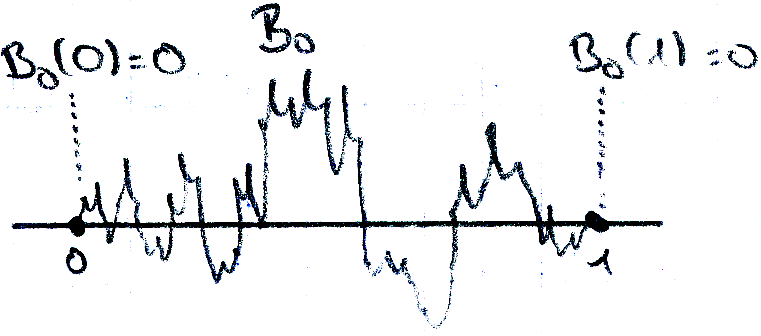
\includegraphics[width=1\textwidth]{./pics/MSTAT002.png}
		\caption{Brownsche Brücke}
		\label{AbbBrownscheBruecke}
	\end{center}
\end{figure}
%Ferger: "Also über die Brücke würde ich jetzt nicht gehen. Kein Ahnung, warum man Brücke dazu sagt."

%T_n^\ast ist Supremumsnorm von Partialsummenprozess?+

Es gilt (vergleiche Shorak und Wellner 1986 \textit{empirical processes}, Seite 34)
\begin{align*}
	H_0(x)&:=\P\left(\sup\limits_{0\leq t\leq 1}\big|B_0(t)\big|\leq x\right)
	\overset{\text{Doob}}{=}
	1-\sum\limits_{k\geq 1}(-1)^{k+1}\cdot\exp\big(-2\cdot k^2\cdot x^2\big)&\forall x>0\\
	H_0(x)&~=0 &\forall x\leq 0
\end{align*}
$H_0$ ist stetig auf $\R$ uns streng monoton auf $[0,\infty)$. 
Folglich ist der Test
\begin{align*}
	H_0\text{ verwerfen }:\Longleftrightarrow T_n^\ast>H_0^{-1}(1-\alpha)
\end{align*}
ist ein asymptotischer Niveau-$\alpha$-Test.\\
$H_0$ ist die Verteilungsfunktion der \textbf{Kolmogorov-Smirnov-Verteilung}.\\
Falls $\mu,\sigma^2$ unbekannt, aber $\nu>\mu$, so betrachte 
\begin{align*}
	\tilde{T}_n&:=\frac{1}{\sqrt{n}}\cdot\frac{1}{\hat{\sigma}_n}\cdot\max\limits_{0\leq k\leq n}\left(\sum\limits_{i=1}^kX_i-\overline{X}_n\right)
\end{align*}
Vollkommen analog folgt: $\tilde{T}_n\stackrel{\L}{\longrightarrow}\sup\limits_{0\leq t\leq 1} B_0(t)$ unter $H_0$. 
Es gilt (vergleiche z.B. Gänssler + Stute (1977) \textit{Wahrscheinlichkeitstheorie}, Seite 322)
\begin{align*}
	H_0^+(x)&:=\P\left(\sup\limits_{0\leq t\leq 1}B_0(t)\leq x\right)=1-\exp\left(-2\cdot x^2\right) &\forall x\geq0\\
	H_0^+(x)&:=0 &\forall x<0
\end{align*}
Da 
\begin{align*}
	(H_0^+)^{-1}(1-\alpha)&=\left(-\frac{1}{2}\cdot\log(\alpha)\right)^{\frac{1}{2}}
\end{align*}
folgt, dass der (einseitige) Test
\begin{align*}
	H_0\text{ verwerfen}:\Longleftrightarrow\tilde{T}_n>\left(-\frac{1}{2}\cdot\log(\alpha)\right)^{\frac{1}{2}}
\end{align*}
ein asymptotischer Niveau-$\alpha$-Test für $H_0$ ist.\nl
Anstelle von
\begin{align*}
	T_n^\ast=\frac{1}{\sqrt{n}}\cdot\frac{1}{\hat{\sigma}_n}\cdot\max\limits_{0\leq k \leq n}\bigg|\underbrace{\sum\limits_{i=1}^k\big(X_i-\overline{X}_n\big)}_{=:C_k}\bigg|
\end{align*}
(die $C_k$ heißen \textbf{kumulierte Summe}) betrachten Csörgő und Horváth (1977) in \textit{Limit Theorems in Change-point Analysis} \ul{gewichtete} kumulierte Summen:
\begin{align*}
	U_n^\ast&:=\sqrt{n}\cdot\frac{1}{\hat{\sigma}_n}\cdot\max\limits_{1\leq k\leq n-1}\frac{|C_k|}{\sqrt{k\cdot(n-k)}}
\end{align*}

\begin{thm}[Csörgő und Horváth]\label{theoremCH} %noNumber
	Seien
	\begin{align*}
		A_n&:=\sqrt{2\cdot\log\big(\log(n)\big)}\\
		D_n&:=2\cdot\log\big(\log(n)\big)+\frac{1}{2}\cdot\log\Big(\log\big(\log(n)\big)\Big)-\frac{1}{2}\cdot\log(\pi)\qquad\forall n\geq n_0
	\end{align*}
	Dann gilt unter $H_0$:
	\begin{align}\label{eqTheoremCsorgoHorvath}\tag{1}
		\limn\P\Big(A_n\cdot U_n^\ast-D_n\leq t\Big)=\exp\big(-2\cdot\exp(-t)\big)=:G(t)
		\qquad\forall t\in\R
	\end{align}
	$G$ ist die sogenannte \textbf{Gumbel-Verteilung}.
\end{thm}

Damit Konstruktion eines asymptotischen Niveau-$\alpha$-Tests für $H_0$ wie folgt möglich: Sei
\begin{align*}
	t_\alpha&:=G^{-1}(1-\alpha)=-\log\left(-\frac{1}{2}\cdot\log(1-\alpha)\right)
\end{align*}
Klarerweise gilt:
\begin{align*}
	A_n\cdot U_n^\ast-D_n>t_\alpha\implies U_n^\ast>\frac{t_\alpha+D_n}{A_n}:=d_n(\alpha)
\end{align*}
Somit ist 
\begin{align*}
	H_0\text{ verwerfen}:\Longleftrightarrow U_n^\ast>d_n(\alpha)
\end{align*}
ein asymptotischer Niveau-$\alpha$-Test, d.h.
\begin{align}\label{eqUnderTheoremCsorgoHarcath}\tag{2}
	\limn\P_{H_0}\big(U_n^\ast>d_n(\alpha)\big)=\alpha
\end{align}
\textbf{Problem:} Die Konvergenz in \eqref{eqTheoremCsorgoHorvath} bzw. in \eqref{eqUnderTheoremCsorgoHarcath} ist sehr sehr sehr laaaaaangsaaaam. %genauso stand das an der Tafel
%Ferger: "[...] Grottenschlecht."
Andererseits führen die Gewichte in $\big(k\cdot(n-k)\big)^{-\frac{1}{2}}$ in $U_n^\ast$ zu einer verbesserten Sensitivität des \textbf{$U_n^\ast$-Test} unter der Alternativen, \underline{insbesondere}, falls $\tau_n$ nahe bei $1$ bzw. oder $n-1$ (am Rand) liegt.\nl
\textbf{Idee:} Weiterhin gewichten, aber durch die \ul{zufällige} Größe $\sqrt{\hat{k}_n\cdot(n-\hat{k}_n)}$ wobei 
\begin{align*}
	\hat{k}_n&:=\min\left\lbrace 1\leq k\leq n:\big|C_k\big|=\max\limits_{1\leq j\leq n-1}\big|C_j\big|\right\rbrace\\
	C_j&:=\sum\limits_{i=1}^j \big(X_i-\overline{X}_n\big)
\end{align*}
d.h. $\hat{k}_n$ ist die kleinste Maximalstelle von $|C_k|,k\in\lbrace1,\ldots,n-1\rbrace$. Erhalte:
\begin{align*}
	R_n=\sqrt{n}\cdot\frac{1}{\hat{\sigma}_n}\cdot\frac{\max\limits_{1\leq k\leq n-1}\left|\sum\limits_{i=1}^k(X_i-\overline{X}_n\big)\right|}{\sqrt{\hat{k}_n\cdot(n-\hat{k}_n)}}
\end{align*}

\begin{thm}[Dietmar Ferger, 2018]%\label{theoremFerger2018} %nonumber
	Sei $(X_i)_{i\in\N}$ eine Folge von i.i.d. Zufallsvariablen mit positiver endlicher Varianz. Dann gilt:
	\begin{align}\label{eqTheoremFerger2018}\tag{3}
		R_n&\stackrel{\L}{\longrightarrow} R
		\qquad\text{wobei}\qquad
		R=\frac{M}{\sqrt{T\cdot(1-T)}}\mit\\
		M&:=\sup\limits_{0\leq t\leq 1}\big|B_0(t)\big|\nonumber,\qquad
		T:=\argmax\limits_{0<t<1}\big|B_0(t)\big|,\qquad
		B_0=\text{ Brownsche Brücke}\nonumber
	\end{align}
\end{thm}

In diesem Theorem %\ref{theoremFerger2018} 
wird die Verteilungsfunktion $H$ von $R$ explizit bestimmt ($H$ hat Reihendarstellung).
%Ferger: "Sie müssen immer eine Anwendung haben. Am besten Sie retten die Welt."
Falls $r_\alpha:=H^{-1}(1-\alpha)$, so liefert \eqref{eqTheoremFerger2018} für den Test
\begin{align*}
	H_0\text{ verwerfen}:\Longleftrightarrow R_n>r_\alpha
\end{align*}
dass gilt:
\begin{align*}
	\limn\P_{H_0}\big(R_n>r_\alpha\big)=\alpha
\end{align*}

\begin{bemerkung}
	\eqref{eqTheoremFerger2018} gilt für $X_{1,n},\ldots,X_{n,n}$ i.i.d. $\forall n\in\N$.\\
	In Simulationsstudien zeigt der $R_n$-Test eine deutlich bessere Güte als der $U_n^\ast$-Test von Csörgő und Horvath.\\
	Falls bekannt ist, dass $\nu>\mu$, so betrachte
	\begin{align*}
		R_n^+&:=\sqrt{n}\cdot\frac{1}{\hat{\sigma}_n}\cdot\frac{\max\limits_{1\leq k\leq n-1}\sum\limits_{i=1}^k\big(X_i-\overline{X}_n\big)}{\sqrt{\hat{k}_n^+\cdot\big(n-\hat{k}_n^+\big)}}\\
		\hat{k}_n^+&:=\min\left\lbrace 1\leq k\leq n-1:C_k=\max\limits_{1\leq j\leq n-1}C_j\right\rbrace
	\end{align*}
\end{bemerkung}

Es gilt:
\begin{align*}
	R_n^+\stackrel{\L}{\longrightarrow} R^+=\frac{M^+}{\sqrt{T^+\cdot(1-T^+)}},\qquad
	M^+=\sup\limits B_0(t),\qquad
	T^*=\argmax\limits B_0(t)\\
	H^+(x):=\P\big(R^+\leq x\big)=2\cdot\Phi(x)-\sqrt{\frac{2}{\pi}}\cdot x\cdot\exp\left(-\frac{1}{2}\cdot x^2\right)-1\qquad x\geq0~(=0, x<0)
\end{align*}
Hierbei ist $\Phi$ die Verteilungsfunktion der Standardnormalverteilung. Ferner gilt:\\
Die Zufallsgrößen $R^+$ und $T^+$ sind stochastisch unabhängig!
\begin{align*}
	\hat{\tau}_n-\tau_n\stackrel{\L}{\longrightarrow}V=\\
	\hat{\tau}_n:=\argmax\limits_{1\leq k\leq n-1}\left|\sum\limits_{i=1}^k\big(X_i-\overline{X_n}\big)\right|
\end{align*}

\subsection{Verteilungskonvergenz in \texorpdfstring{$C(\R)$}{C(R)}}
Häufig hat man mit stochastischen Prozessen zu tun, deren Pfade in
\begin{align*}
	C(\R):=\Big\lbrace f:\R\to\R:f\text{ stetig}\Big\rbrace
\end{align*}
liegen (siehe Beispiel Median ganz am Anfang). Die bisherige Theorie für $C(I)$, $I$\\ \underline{kompaktes} Intervall deckt das nicht ab. Wir versehen $C(\R)$ mit der Metrik
\begin{align*}
	d(f,g)&:=\sum\limits_{j\geq 1} 2^{-j}\cdot\frac{d_j(f,g)}{1+d_j(f,g)} &\forall f,g\in C(\R)\\
	d_j(f,g)&:=\sup\limits_{-j\leq t\leq j}\Big|f(t)-g(t)\Big| &\forall f,g\in C(\R)
\end{align*}
Es zeigt sich, das $\big(C(\R),d\big)$ ein vollständiger separabler metrischer Raum ist. Ferner gilt:
\begin{align*}
	d(f_n,f)\stackrel{n\to\infty}{\longrightarrow}0
	\Longleftrightarrow \forall j\in\N: d_j(f_n,f)\stackrel{n\to\infty}{\longrightarrow}0
	\Longleftrightarrow\text{ glm. Konvergenz auf Kompakta}
\end{align*}
Seien $\pi_t:C(\R)\to R$ und $\pi_T:C(\R)\to\R^{|T|}$ die Projektionsabbildungen, d.h. z.B.
\begin{align*}
	\pi_T(f)=\big(f(t)\big)_{t\in T}=\Big(f(t_1),\ldots,f(t_k)\Big)\qquad
	T=\lbrace t_1,\ldots, t_k\rbrace
\end{align*}

\begin{theorem}\label{theorem7.20}
	\begin{align*}
		\B_d\big(C(\R)\big)&=\sigma\Big(\pi_t:t\in\R\Big)=\sigma\Big(\pi_T:T\subseteq\R\text{ endlich}\Big)
	\end{align*}
\end{theorem}

\begin{proof}
	Die Argumente im Beweis von Satz \ref{satz7.2} lassen sich problemlos übertragen.
\end{proof}

Ebenfalls analog beweist man:

\begin{satz}\label{satz7.21}
	 Sei $(\Omega,\A)$ messbarer Raum und $C:=C(\R)$ versehen mit $\B_d(C)$.\\
	 Dann gilt für eine Abbildung $X:\Omega\to C(\R):$
	 \begin{align*}
	 	X~\A\text{-}\B_d(C)\text{-messbar}
	 	\Longleftrightarrow\forall t\in\R:
	 	\pi_t\circ X~\A\text{-}\B(\R)\text{-messbar }
	 \end{align*}
\end{satz}

Konsequenz aus Satz \ref{satz7.21}: Jeder stetige stochastische Prozess indiziert nach $\R$ kann aufgefasst werden als Zufallsvariable in $(C,d)$.

\begin{satz}\label{satz7.22}
	Seien $X,Y$ Zufallsvariablen in $\big(C(\R),d\big)$. Dann gilt:
	\begin{align*}
		X\stackeq{\L}Y\Longleftrightarrow
		\Big(X(t_1),\ldots,X(t_k)\Big)\stackeq{\L}\Big(Y(t_1),\ldots,Y(t_k)\Big)
	\end{align*}
	für jede Wahl von Punkten $t_1<\ldots<t_k$ aus $\R$.
\end{satz}

\begin{proof}
	Siehe Theorem \ref{theorem7.20} + Maßeindeutigkeitssatz.
\end{proof}

Für $f\in C(\R)$ sei
\begin{align*}
	f^{(j)}:=f|_{[-j,j]},\qquad I_j:=[-j,j]\text{ d.h.}\\
	f^{(j)}:I_j\to\R,\qquad f^{(j)}(t):=f(t)\qquad\forall t\in I_j
\end{align*}

\begin{satz}\label{satz7.23}
	Seien $X,X_n,n\in\N$ Zufallsvariablen in $\big(C(\R),d\big)$. Dann gilt:
	\begin{align*}
		X_n\stackrel{\L}{\longrightarrow}X\text{ in }\big(C(\R),d\big)
		\Longleftrightarrow\forall j\in\N:
		X_n^{(j)}\stackrel{\L}{\longrightarrow} X^{(j)}\text{ in }\big(C(I_j),d_j\big)
	\end{align*}
\end{satz}

Satz \ref{satz7.23} geht auf Whitt (1970) zurück. Ein (relativ) einfacher Beweis findet sich in Kallenberg (1997), \textit{Foundations of modern probability}, Seite 260.

\begin{bemerkungnr}\label{bemerkung7.24}\
	\begin{enumerate}[label=(\arabic*)]
		\item Die Resultate in \ref{theorem7.20},\ref{satz7.21},\ref{satz7.22} und \ref{satz7.23} gelten analog für $C\big([0,\infty)\big)$ mit $I_j$ ersetzt durch $[0,j]$.
		\item Satz \ref{satz7.23} ermöglicht es insbesondere, auf die Konvergenz-Kriterien in \ref{satz7.9} und \ref{satz7.11MomentenkriteriumVonKolmogoroff} zurückzugreifen.
	\end{enumerate}
\end{bemerkungnr}

\begin{beispiel}\label{beispiel7.25}
	 Seien $(\xi_i)_{i\in\N}$ i.i.d. mit $\E[\xi_1]=0$, $\Var(\xi_1)=1$ und 
	 \begin{align*}
	 	S_k&:=\sum\limits_{j=1}^k\xi_j\qquad\forall k\in\N_0\\
	 	X_n(t)&:=\frac{1}{\sqrt{n}}\cdot S_{\lceil n\cdot t\rceil}+\frac{1}{\sqrt{n}}\cdot\big(n\cdot t-\lceil n\cdot t\rceil\big)\cdot\xi_{\lceil n\cdot t\rceil+1}\qquad\forall t\in[0,\infty)
	 \end{align*}
	 D.h. $X_n$ ist Polygonzug durch $\left(\frac{k}{n},\frac{1}{\sqrt{n}\cdot S_n}\right),k\in\N_0$.
	 Aus Satz \ref{satz7.16Donsker} folgt:
	 \begin{align*}
	 	&X_n^{(j)}\stackrel{\L}{\longrightarrow}B^{(j)}\qquad\forall j\in\N\\
	 	&\overset{\ref{bemerkung7.24}(1)+\ref{satz7.23}}&\Longleftrightarrow
	 	X_n\stackrel{\L}{\longrightarrow} B\text{ in }\Big(C\big([0,\infty)\big),d\Big)
	 \end{align*}
\end{beispiel}